\chapter{ISAC-Enabled Multi-device Multi-target Cooperative Sensing: A Fairness-Aware Design}
\label{chap4_iotj}

\section{Introduction} \label{chap4_sec_introduction}

With the deep convergence of the Internet of Things (IoT), artificial intelligence and communication networks, future 6G wireless networks are evolving rapidly to deliver comprehensive and immersive services \cite{iotj.10185562,intro.10292797,iotj.10361270}. The emergence of immersive services in 6G networks, such as autonomous driving, extended reality and digital twins, imposes stringent demands for both ultra-reliable low-latency transmission and high-precision localization \cite{iotj.fadlullah2021smart}. Integrated sensing and communication (ISAC), which enables simultaneous data transmission and sensing information collection via integrated signals over the same spectrum, has been recognized as a spectrum-efficient paradigm to address the conflict between these growing demands and limited wireless resources, and thus attracts wide research interests \cite{iotj.10233699,intro.9842350,intro.10050406,intro.10147248,intro.10630588}. Due to the great potential of ISAC in improving the spectrum efficiency and resource utilization, it has been expected to serve as an enabling technology in numerous future application scenarios, such as intelligent transportation and intelligent manufacturing.

Existing literature has explored deploying ISAC on wireless devices to acquire accurate environmental information, leveraging their wide distribution and proximity to targets \cite{iotj.9796610,iotj.liu2022vertical,iotj.ding2022joint,intro.10273396}. Nevertheless, the performance of ISAC in single-device systems is fundamentally constrained by stringent hardware resources and limited sensing apertures, particularly in multi-target scenarios. Furthermore, managing the mutual interference between communication and multi-target sensing poses significant challenges for resource allocation within a single device.
To overcome these limitations, leveraging multi-device cooperative sensing has emerged as a promising solution. By exploiting the spatial diversity of distributed devices, cooperative sensing allows multiple nodes to jointly accomplish sensing tasks, thereby alleviating the resource bottlenecks faced by individual devices. Moreover, sensing from diverse spatial locations yields more comprehensive environmental reconstruction and mitigates performance degradation caused by potential shadowing or blockage. In this context, this chapter considers a framework where devices perform cooperative sensing in a time-division manner, allowing each device to execute ISAC functions without inter-device interference.
However, time-division access introduces a critical fairness concern. In cooperative networks, allocating time resources to maximize system-wise performance often leads to the over-exploitation of devices with superior channel conditions, while others are starved. Designing fairness-aware mechanisms is therefore crucial to achieving balanced performance and prolonging network lifetime, yet efficiently utilizing heterogeneous resources across different devices remains a challenge. Additionally, achieving a flexible trade-off between data transmission and high-precision sensing in multi-target scenarios with diverse requirements remains an open issue.

To address these challenges, this chapter proposes a fairness-aware ISAC-enabled multi-device cooperative sensing framework. We investigate a joint optimization of time allocation and transceiver beamforming, aiming to balance system-wise throughput with individual device fairness. The main contributions of this chapter are summarized as follows.
\begin{itemize}
	\item We propose a fairness-aware ISAC-enabled multi-device cooperative sensing system in which the devices engage in cooperative sensing towards multiple targets in a time-division manner. Within the allocated time, each device senses the targets and transmits data to the base station simultaneously via ISAC.
	We formulate a joint optimization of the beamforming for both sensing and transmission as well as the time allocation for different devices, aiming at maximizing the total throughput of the devices while guaranteeing the multi-target sensing quality, the cooperative sensing requirement and the fairness in data transmission.
	\item To tackle the non-convexity of the problem, we decompose it into a subproblem for beamforming optimization and a subproblem for time allocation via the block coordinate descent. For the beamforming optimization subproblem, we first analyze the necessity of the additional dedicated sensing signal. Then, we present a convex surrogate problem for the non-convex subproblem by designing surrogate functions, and obtain the solution of the beamforming via the successive convex approximation method. For the time allocation subproblem, we analyze the feature of the optimal time allocation for different devices while providing the semi-analytical expression. 
	\item We present the simulation results to verify the effectiveness of our proposed algorithm. Compared with several benchmark algorithms, our algorithm achieves a superior performance. Moreover, simulation results validate the performance advantages of our fairness-aware ISAC-enabled cooperative sensing scheme. Compared with several benchmark schemes, our fairness-aware ISAC-enabled cooperative sensing scheme outperforms other benchmark schemes in both throughput and cooperative sensing accuracy.
\end{itemize}

The remainder of the chapter is organized as follows. Section \ref{chap4_sec_systemmodel} illustrates the system model and problem formulation. In Section \ref{chap4_sec_convergenceformulation}, show the problem decomposition and identify the solution features of the decomposed subproblems. We further propose an efficient algorithm for solving the formulated problem in Section \ref{chap4_sec_convergenceformulation}. Section \ref{chap4_sec_result} demonstrates the performance of our fairness-aware ISAC-enabled multi-device cooperative sensing and Section \ref{chap4_sec_conclusion} conclude this chapter.


\textit{Notations:} The trace of matrix $\mathbf{I}$ is denoted by $\mathbf{Tr}(\mathbf{I})$. The transpose of matrix $\mathbf{I}$ is denoted by $\mathbf{I}^T$. The conjugate transpose of matrix $\mathbf{I}$ is denoted by $\mathbf{I}^H$. The conjugate of matrix $\mathbf{I}$ is denoted by $\mathbf{I}^\dagger$. $\mathrm{Re}\{\cdot\}$ denotes the real part of a complex value. $||\cdot||_F^2$ denotes the square of Frobenius-norm.

\section{System Model of ISAC-Enabled Cooperative Sensing} \label{chap4_sec_systemmodel}

\begin{figure}
   \centering
   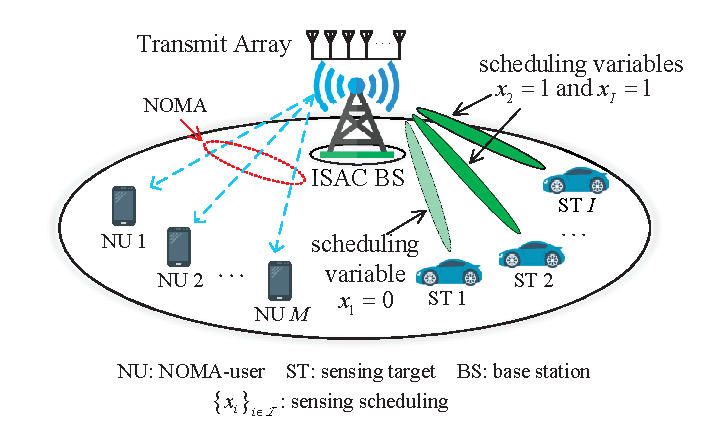
\includegraphics[width=0.9\textwidth]{figs_iotj_cld/Figure1.eps}
   \caption{An illustrative system model}\label{fig:figure_model41}
\end{figure}

Figure \ref{fig:figure_model41} illustrates the system model of our ISAC-enabled multi-device cooperative sensing. There exists a group of integrated sensing and communication devices (SCDs) with $N_t$ transmit antennas and $N_r$ receive antennas denoted by $\mathcal{K}=\{1,2,...,K\}$. All SCDs perform cooperative sensing of a group of given targets which are denoted by $\mathcal{M}=\{1,2,...,M\}$ in a time-division multiple-access manner, with each SCD sensing the targets as well as transmitting data to the base station (BS) simultaneously within its allocated time. We model the cooperative sensing as a $K$-phase process, where we allocate time $t_k$ to SCD $k$ at Phase $k$.

\subsection{Modeling of Phase $k$}
	
In Phase $k$, the integrated signal of SCD $k$ for delivering its data to the BS and sensing the targets can be expressed as
\begin{equation}
	\mathbf{x}_{k}=\mathbf{u}_{k}z_{k}+\mathbf{v}_{k},
	\label{transmit_k}
\end{equation}
where $\mathbf{u}_{k}\in\mathbb{C}^{N_t\times 1}$ denotes the SCD $k$'s transmit beamforming vector for the BS, and $z_{k}$ denotes the data symbol of SCD $k$. Vector $\mathbf{v}_{k}$ denotes the dedicated sensing signal of SCD $k$. The received signal at the BS within Phase $k$ is given by
\begin{equation}
	y_{k}^{\text{BS}}=\mathbf{g}_k^H\mathbf{u}_{k}z_{k}+\mathbf{g}_k^H\mathbf{v}_{k}+n_0,
	\label{receive_bs_k}
\end{equation}
where $\mathbf{g}_k\in\mathbb{C}^{N_t\times 1}$ denotes the channel gain between the BS and SCD $k$, and $n_0$ denotes the noise at the BS with variance $\sigma_{0}^2$.

We next model the sensing channel for SCD $k$ regarding the targets. Assume that both the transmit and receive uniform linear arrays are half-wavelength antenna spacing. Then, the transmit steering vector and the receive steering vector on direction $\theta$ are respectively given by
\begin{equation}
	\mathbf{a}_t(\theta)=\frac{1}{\sqrt{N_t}}\left[1,e^{j\pi \sin\theta},...,e^{j\pi (N_t-1)\sin\theta}\right]^T,
\end{equation}
\vspace{0.5cm}
\begin{equation}
	\mathbf{a}_r(\theta)=\frac{1}{\sqrt{N_r}}\left[1,e^{j\pi \sin\theta},...,e^{j\pi (N_r-1)\sin\theta}\right]^T.
\end{equation}
The received signal at SCD $k$ within Phase $k$ consists of three parts, including the sensing echoes from the desired targets with the direction of $\{\theta_{km}\}_{m\in\mathcal{M}}$, the clutter interference from $J$ undesired clutters under the direction $\{\theta_{kj}\}_{j\in\mathcal{J}}$, and the self-interference and noise.
We consider that the SCDs have prior knowledge of the targets and clutters. Therefore, we express the received signal at SCD $k$ within Phase $k$ as 
\begin{equation}
	\begin{split}
	\mathbf{y}_{k}^{\text{ID}}=&\mathop{\underbrace{\sum_{m\in\mathcal{M}}\beta_{km}\mathbf{a}_r(\theta_{km})\mathbf{a}_t^H(\theta_{km})\mathbf{x}_{k}}\limits_{\text{sensing echoes from $M$ desired targets}}}+\\&\mathop{\underbrace{\sum_{j\in\mathcal{J}}\beta_{kj}\mathbf{a}_r(\theta_{kj})\mathbf{a}_t^H(\theta_{kj})\mathbf{x}_{k}}\limits_{\text{clutter interference from $J$ undesired targets}}}+\mathop{\underbrace{\mathbf{H}_k^{\text{SI}}\mathbf{x}_k+\mathbf{n}_{k}}\limits_{\text{self-interference and noise}}}, 
	\end{split}
	\label{receive_device_k}
\end{equation}
where $\beta_{km}$ is the complex amplitude of target $m$ regarding SCD $k$. The value of $\beta_{km}$ is mainly determined by the path loss and the radar cross-section. Vector $\mathbf{H}_k^{\text{SI}}\in\mathbb{C}^{N_r\times N_t}$ denotes the residual self-interference channel at SCD $k$, and $\mathbf{n}_{k}$ denotes the noise with variance $\sigma_{k}^2$. In the following context, we define $\mathbf{A}_{km}\triangleq \beta_{km}\mathbf{a}_r(\theta_{km})\mathbf{a}_t^H(\theta_{km})$, and $\mathbf{A}_{k}^{\text{ITF}}\triangleq \sum_{j\in\mathcal{J}}\beta_{kj}\mathbf{a}_r(\theta_{kj})\mathbf{a}_t^H(\theta_{kj})+\mathbf{H}_k^{\text{SI}}$.


Based on eq. (\ref{receive_bs_k}), the achievable data transmission rate $R_{k}$ from SCD $k$ to the BS is expressed as
\begin{equation}
	R_{k}=B\log_2\left(1+\frac{|\mathbf{g}_{k}^H\mathbf{u}_{k}|^2}{|\mathbf{g}_{k}^H\mathbf{v}_{k}|^2+\sigma_{0}^2}\right), \label{Rk}
\end{equation}
where $B$ denotes the channel bandwidth. 
The covariance of SCD $k$'s transmitted signal is given by
\begin{equation}
	\mathbf{W}_k=\mathbb{E}(\mathbf{x}_k\mathbf{x}_k^H)=\mathbf{u}_k\mathbf{u}_k^H+\mathbf{v}_k\mathbf{v}_k^H.
\end{equation}
We measure the multi-target sensing performance by using beampattern matching error and mean-squared cross correlation \cite{iotj.stoica2007probing}. Specifically, the beampattern matching error quantifies the disparity between the desired radiation pattern and the actual measured pattern. Let $\{\psi(\theta_{kq})\}_{q=1}^{Q}$ denote the pre-designed beampattern of SCD $k$, the SCD $k$'s beampattern matching error between the obtained beampattern and the pre-designed beampattern is given by
\begin{equation}
	\xi_k=\frac{1}{Q}\sum_{q=1}^{Q}|\varsigma_k \psi(\theta_{kq})-\mathbf{a}_t^H(\theta_{kq})\mathbf{W}_k\mathbf{a}_t(\theta_{kq})|^2, 
\end{equation}
where $\varsigma_k$ is the scaling factor of SCD $k$ and $\{\theta_{kq}\}_{q=1}^{Q}$ are the sampled angle grids. The mean-squared cross correlation is used to quantify the correlation between two signals. For high-quality multi-target sensing, there should be a significant difference between the signals in different target directions, i.e., a low cross correlation value should be held, which facilitates the effective separation and extraction of the sensing echoes from different directions. The mean-squared cross correlation of SCD $k$'s transmit signal is given by
\vspace{0.3cm}
\begin{equation}
	\zeta_k=\frac{2}{M^2-M}\sum_{i=1}^{M}\sum_{i^{'}=i+1}^{M}|\mathbf{a}_t^H(\theta_{ki})\mathbf{W}_k\mathbf{a}_t(\theta_{ki^{'}})|^2, \label{zeta}
\end{equation}

\vspace{-1cm}
We measure the cooperative sensing performance by using the sensing estimation rate, which is defined as the cancellation of the uncertainty in the target parameters per second. Based on eq. (\ref{receive_device_k}), the sensing estimation rate $S_{k}$ of SCD $k$ for sensing target $m$ is characterized as
\begin{equation}
	S_{km}=\frac{\delta}{2\mu}\log_2\left(1+\frac{2\mu B\mathbf{c}_{km}^H\mathbf{A}_{km}\mathbf{W}_{k}\mathbf{A}_{km}^H\mathbf{c}_{km}}{\mathbf{c}_{km}^H\mathbf{\Lambda}_{km}\mathbf{c}_{km}}\right), \label{estimation}
\end{equation}
where $\delta$ denotes the radar duty factor, and $\mu$ denotes the radar pulse duration. Vector $\mathbf{c}_{km}\in\mathbb{C}^{N_r \times 1}$ denotes the receive beamforming of SCD $k$ for sensing target $m$. Vector $\mathbf{\Lambda}$ is the interference of SCD $k$ for sensing target $m$, and it can be expressed as
\begin{equation}
	\mathbf{\Lambda}_{km}=\mathbf{A}_{k}^{\text{ITF}}\mathbf{W}_k(\mathbf{A}_{k}^{\text{ITF}})^H+\sum_{m^{'}\neq m}\mathbf{A}_{km^{'}}\mathbf{W}_k\mathbf{A}_{km^{'}}^H+\sigma_k^2\mathbf{I}_N.
\end{equation}
According to \cite{twc1.van2002optimum}, the optimal receivers $\mathbf{c}_{km}^*$ is given by
\begin{equation}
		\mathbf{c}_{km}^*=\arg\max\frac{\mathbf{c}_{km}^H\mathbf{A}_{km}\mathbf{W}_{k}\mathbf{A}_{km}^H\mathbf{c}_{km}}{\mathbf{c}_{km}^H\mathbf{\Lambda}_{km}\mathbf{c}_{km}}=\mathbf{\Lambda}_{km}^{-1}\mathbf{a}_r(\theta_{km}).
	\label{optimal_receiver}
\end{equation}
By substituting eq. (\ref{optimal_receiver}) into eq. (\ref{estimation}), we can rewrite $S_{km}$ as

\begin{equation}
	S_{km}=\frac{\delta}{2\mu}\log_2\left(1+2\mu B\mathbf{x}_{k}^H\mathbf{A}_{km}^H\mathbf{\Lambda}_{km}^{-1}\mathbf{A}_{km}\mathbf{x}_{k}\right). \label{Skm}
\end{equation}



\subsection{Problem Formulation}

We aim at maximizing the total throughput of the SCDs considering the fairness (MTCF), while guaranteeing the requirements of both multi-target sensing and cooperative sensing for the given targets. To this end, we conduct a joint optimization of the SCDs' beamforming vectors $\{\mathbf{u}_k\}_{k\in\mathcal{K}}$, $\{\mathbf{v}_k\}_{k\in\mathcal{K}}$, and the time allocation $\{t_{k}\}_{k\in\mathcal{K}}$.
\begin{flalign}
	\text{(MTCF):~}
	&\max  \sum_{k\in\mathcal{K}}\ln(R_k t_k)\nonumber\\
	\text{subject to:~}
	&\sum_{k\in\mathcal{K}}t_k\le T, t_k\ge 0, \label{iotj.con1}
	\\
	&\sum_{k\in\mathcal{K}}S_{km}t_k\ge S_m^{\text{req}}, \forall m\in\mathcal{M}, \label{iotj.con2}
	\\
	&\xi_k\le \xi^{\text{max}}, \forall k\in\mathcal{K}, \label{iotj.con3}
	\\
	&\zeta_k\le \zeta^{\text{max}}, \forall k\in\mathcal{K}, \label{iotj.con4}
	\\
	&\mathbf{Tr}(\mathbf{W}_k)\le P_k^{\text{max}}, \forall k\in\mathcal{K}, \label{iotj.con5}
	\\
	\text{variables:~} & {\{\mathbf{u}_k\}_{k\in\mathcal{K}}}, {\{\mathbf{v}_k\}_{k\in\mathcal{K}}}, \text{~and~} {\{t_k\}_{k\in\mathcal{K}}}.\nonumber
\end{flalign}
In the objective function, we use $\ln(\cdot)$ function as the utility of SCD $k$ for delivering its data volume in Phase $k$, and maximize the total utility of the SCDs. This objective function facilitates the fairness of the throughput of different devices, which leads to a balanced allocation of data transmission opportunities. Constraint (\ref{iotj.con1}) ensures that the total time allocation cannot exceed the maximum time $T$. Constraint (\ref{iotj.con2}) guarantees the minimum cooperative sensing requirement $S_m^{\text{req}}$ for arbitrary target $m$. Constraint (\ref{iotj.con3}) ensures that the beampattern matching error of SCD $k$ cannot exceed the maximum error $\xi^{\text{max}}$. Constraint (\ref{iotj.con4}) ensures that the value of mean-squared cross correlation of SCD $k$'s transmit signal cannot exceed a required level $\zeta^{\text{max}}$. Constraints (\ref{iotj.con3}) and (\ref{iotj.con4}) guarantee the SCD $k$'s multi-target sensing performance. Constraint (\ref{iotj.con5}) ensures that the total power consumption of SCD $k$ cannot exceed its power capacity $P_k^{\text{max}}$.


\section{Proposed Algorithms for Solving Problem (MTCF)} \label{chap4_sec_convergenceformulation}

\subsection{Decomposition of Problem (MTCF)}

Problem (MTCF) is a strictly non-convex optimization problem since the beamforming variables and time allocation variables are coupled in both the objective function and constraints, which is difficult to solve directly. To address this issue, we first decompose the original Problem (MTCF) into two subproblems, including a subproblem for beamforming optimization (BO) and a subproblem for time allocation (TA), which are shown as follows.
\begin{flalign}
	\text{(MTCF-BO):~}
	&\max  \sum_{k\in\mathcal{K}}\ln(R_k t_k)\nonumber\\
	\text{subject to:~}
	&\text{constraints~} (\ref{iotj.con2}), (\ref{iotj.con3}), (\ref{iotj.con4}) \text{~and~} (\ref{iotj.con5}),\nonumber
	\\
	\text{variables:~} & {\{\mathbf{u}_k\}_{k\in\mathcal{K}}} \text{~and~} {\{\mathbf{v}_k\}_{k\in\mathcal{K}}}.\nonumber
	\\\nonumber
	\\
	\text{(MTCF-TA):~}
	&\max  \sum_{k\in\mathcal{K}}\ln(R_k t_k)\nonumber\\
	\text{subject to:~}
	&\text{constraints~} (\ref{iotj.con1}) \text{~and~} (\ref{iotj.con2}),\nonumber
	\\
	\text{variables:~} & {\{t_k\}_{k\in\mathcal{K}}}.\nonumber
\end{flalign}
Then, we solve the two subproblems iteratively by adopting the block coordinate descent method. The details for solving these two subproblems are shown in Section 4.3.2 and Section 4.3.3.

\subsection{Algorithm for Solving Problem (MTCF-BO)}

Problem (MTCF-BO) is still a strictly non-convex problem since the objective function and constraints (\ref{iotj.con2})-(\ref{iotj.con4}) are non-convex. We first identify the solution feature of $\mathbf{v}_k$ as follows.

\begin{proposition}
	\label{proposition7}
	The optimal solution of Problem (MTCF-BO) has the feature as
	\begin{equation}
		\{\mathbf{v}_k^*\}_{k\in\mathcal{K}}=\mathbf{0}.
	\end{equation}
\end{proposition}
\begin{proof}
	We consider Problem (MTCF-BO), which is under the given ${\{\mathbf{u}_k\}_{k\in\mathcal{K}}}$, as follows
\begin{flalign}
	\text{(BO-v):~}
	&\max  \sum_{k\in\mathcal{K}}\ln\left(t_kB\log_2\left(1+\frac{|\mathbf{g}_{k}^H\mathbf{u}_{k}|^2}{|\mathbf{g}_{k}^H\mathbf{v}_{k}|^2+\sigma_{0}^2}\right)\right)\nonumber\\
	\text{subject to:~}
	&\text{constraints~} (\ref{iotj.con2}), (\ref{iotj.con3}), (\ref{iotj.con4}) \text{~and~} (\ref{iotj.con5}),\nonumber
	\\
	\text{variables:~} & {\{\mathbf{v}_k\}_{k\in\mathcal{K}}}.\nonumber
\end{flalign}
We notice the following important features. On the one hand, the objective function aims to minimize ${\{|\mathbf{g}_k^H\mathbf{v}_k|^2\}_{k\in\mathcal{K}}}$ and maximize ${\{|\mathbf{g}_k^H\mathbf{u}_k|^2\}_{k\in\mathcal{K}}}$. On the other hand, ${\{\mathbf{u}_k\}_{k\in\mathcal{K}}}$ and ${\{\mathbf{v}_k\}_{k\in\mathcal{K}}}$ play the same role in constraints (\ref{iotj.con2})-(\ref{iotj.con5}), i.e., for arbitrary ${\{\mathbf{v}_k\}_{k\in\mathcal{K}}}\neq \mathbf{0}$, we can transfer its power to ${\{\mathbf{u}_k\}_{k\in\mathcal{K}}}$ without changing the feasible region constituted by constraints (\ref{iotj.con2})-(\ref{iotj.con5}). Therefore, we can conclude that the optimal solution of ${\{\mathbf{v}_k\}_{k\in\mathcal{K}}}$ in Problem (MTCF-BO) is ${\{\mathbf{v}_k^*\}_{k\in\mathcal{K}}=\mathbf{0}}$.
\end{proof}
Proposition \ref{proposition7} implies that the communication signal can be entirely repurposed for sensing, without the necessity to design the additional dedicated sensing signal for this scenario, which can simplify the system design of the ISAC device and the deployment of the ISAC system in practical applications. By substituting this solution into Problem (MTCF-BO), we can derive the following problem
\begin{flalign}
	\text{(BO-E):~}
	&\max  \sum_{k\in\mathcal{K}}\ln\left(t_kB\log_2\left(1+\frac{\mathbf{u}_{k}^H\mathbf{G}_{k}\mathbf{u}_{k}}{\sigma_{0}^2}\right)\right)\nonumber\\
	\text{subject to:~}
	&\text{constraints~} (\ref{iotj.con2}), (\ref{iotj.con3}), (\ref{iotj.con4}) \text{~and~} (\ref{iotj.con5}),\nonumber
	\\
	\text{variables:~} & {\{\mathbf{u}_k\}_{k\in\mathcal{K}}}.\nonumber
\end{flalign}
In Problem (BO-E), we define $\mathbf{G}_k\triangleq\mathbf{g}_k\mathbf{g}_k^H$, and $\mathbf{W}_k$ is rewritten as $\mathbf{W}_k=\mathbf{u}_k\mathbf{u}_k^H$. Next, we use successive convex approximation (SCA) to address the non-convexity of the objective function and constraints (\ref{iotj.con2})-(\ref{iotj.con4}), and thus transform Problem (BO-E) into a tractable form.

\begin{proposition}
	\label{proposition8}
	$S_{km}$ in eq. (\ref{Skm}) can be equivalently transformed into $\hat{S}_{km}$ as follows

	\begin{equation}
		\begin{split}
		\hat{S}_{km}=&2\sqrt{{\delta B}(1+\gamma_{km})}\mathrm{Re}\{\mathbf{u}_k^H\mathbf{A}_{km}^H\mathbf{f}_{km}\}-2\mu B||\mathbf{f}_{km}^H\mathbf{A}_{km}\mathbf{u}_k||_F^2-||\mathbf{f}_{km}^H\mathbf{A}_{k}^{\mathrm{ITF}}\mathbf{u}_k||_F^2\\&-\sum_{m^{'}\neq m}||\mathbf{f}_{km}^H\mathbf{A}_{km^{'}}\mathbf{u}_k||_F^2-\sigma_k^2||\mathbf{f}_{km}||_F^2+\frac{\delta}{2\mu}\log_2(1+\gamma_{km})-\frac{\delta}{2\mu}\gamma_{km},
		\end{split}
		\label{SCA_S}
	\end{equation}
	where $\{\gamma_{km}\}_{k\in\mathcal{K},m\in\mathcal{M}}$ and $\{\mathbf{f}_{km}\}_{k\in\mathcal{K},m\in\mathcal{M}}$ are auxiliary variables and their optimal values can be given by
	\begin{equation}
		\gamma_{km}^*=2\mu B\mathbf{u}_k^H\mathbf{A}_{km}^H\mathbf{\Lambda}_{km}^{-1}\mathbf{A}_{km}\mathbf{u}_k, \label{gammakm}
	\end{equation}
	\begin{equation}
		\mathbf{f}_{km}^*\hspace{-0.1cm}=\hspace{-0.1cm}\sqrt{{\delta B}(1+\gamma_{km})}(2\mu B\mathbf{A}_{km}\mathbf{u}_k\mathbf{u}_k^H\mathbf{A}_{km}^H+\mathbf{\Lambda}_{km})^{\hspace{-0.05cm}-\hspace{-0.05cm}1}\hspace{-0.1cm}\mathbf{A}_{km}\mathbf{u}_k. \label{fkm}
	\end{equation}
\end{proposition}
\vspace{-1cm}
\begin{proof}
	By using Lagrangian dual transform method, we introduce the auxiliary variables $\{\gamma_{km}\}_{k\in\mathcal{K},m\in\mathcal{M}}$ and rewrite $S_{km}$ in eq. ({\ref{Skm}}) as
\begin{equation}
	\begin{split}
	\tilde{S}_{km}={\delta B}(1+\gamma_{km})\mathbf{u}_k^H\mathbf{A}_{km}^H\mathbf{D}_{km}^{-1}\mathbf{A}_{km}\mathbf{u}_k+\frac{\delta}{2\mu}\log_2(1+\gamma_{km})-\frac{\delta}{2\mu}\gamma_{km},
	\end{split}
	\label{tildeSkm}
\end{equation}
where $\mathbf{D}_{km}$ is given by
\begin{equation}
	\mathbf{D}_{km}=2\mu B\mathbf{A}_{km}\mathbf{u}_k\mathbf{u}_k^H\mathbf{A}_{km}^H+\mathbf{\Lambda}_{km}. \label{Dkm}
\end{equation}
It can be identified that $\tilde{S}_{km}$ is a concave function of $\{\gamma_{km}\}_{k\in\mathcal{K},m\in\mathcal{M}}$ under the given $\{\mathbf{u}_k\}_{k\in\mathcal{K}}$ \cite{twc1.boyd2004convex}. The first derivative of $\tilde{S}_{km}$ regarding $\{\gamma_{km}\}_{k\in\mathcal{K},m\in\mathcal{M}}$ is given by
\begin{equation}
	\frac{\partial \tilde{S}_{km}}{\gamma_{km}}={\delta B}\mathbf{u}_k^H\mathbf{A}_{km}^H\mathbf{D}_{km}^{-1}\mathbf{A}_{km}\mathbf{u}_k-\frac{\delta\gamma_{km}}{2\mu(1+\gamma_{km})}. \label{gamma_partial}
\end{equation}
By using Sherman-Morrison formula, eq. (\ref{gamma_partial}) can be rewritten as
\begin{equation}
	\begin{split}
	\frac{\partial \tilde{S}_{km}}{\gamma_{km}}&=-\frac{2\mu\delta B^2\mathbf{u}_k^H\mathbf{A}_{km}^H\mathbf{\Lambda}_{km}^{-1}\mathbf{A}_{km}\mathbf{u}_k\mathbf{u}_k^H\mathbf{A}_{km}^H\mathbf{\Lambda}_{km}^{-1}\mathbf{A}_{km}\mathbf{u}_k}{1+2\mu B\mathbf{u}_k^H\mathbf{A}_{km}^H\mathbf{\Lambda}_{km}^{-1}\mathbf{A}_{km}\mathbf{u}_k}\\&~+{\delta B}\mathbf{u}_k^H\mathbf{A}_{km}^H\mathbf{\Lambda}_{km}^{-1}\mathbf{A}_{km}\mathbf{u}_k-\frac{\delta\gamma_{km}}{2\mu(1+\gamma_{km})}\\&=\frac{\delta B\mathbf{u}_k^H\mathbf{A}_{km}^H\mathbf{\Lambda}_{km}^{-1}\mathbf{A}_{km}\mathbf{u}_k}{1+2\mu B\mathbf{u}_k^H\mathbf{A}_{km}^H\mathbf{\Lambda}_{km}^{-1}\mathbf{A}_{km}\mathbf{u}_k}-\frac{\delta\gamma_{km}}{2\mu(1+\gamma_{km})}.
	\end{split}
\end{equation}
By setting $\frac{\partial \tilde{S}_{km}}{\gamma_{km}}=0$, we can derive that the optimal solution of $\{\gamma_{km}\}_{k\in\mathcal{K},m\in\mathcal{M}}$ can be expressed as
\begin{equation}
	\gamma_{km}^*=2\mu B\mathbf{u}_k^H\mathbf{A}_{km}^H\mathbf{\Lambda}_{km}^{-1}\mathbf{A}_{km}\mathbf{u}_k.
\end{equation}
Since eq. (\ref{tildeSkm}) is still non-convex, we further use multi-dimensional quadratic transform method \cite{iotj.shen2018fractional} to rewrite $\tilde{S}_{km}$ as
\begin{equation}
	\begin{split}
	\hat{S}_{km}=&2\sqrt{{\delta B}(1+\gamma_{km})}\text{Re}\{\mathbf{u}_k^H\mathbf{A}_{km}^H\mathbf{f}_{km}\}-\mathbf{f}_{km}^H\mathbf{D}_{km}\mathbf{f}_{km}\\&+\frac{\delta}{2\mu}\log_2(1+\gamma_{km})-\frac{\delta}{2\mu}\gamma_{km},
	\end{split}
	\label{hatSkm}
\end{equation}
where $\{\mathbf{f}_{km}\}_{k\in\mathcal{K},m\in\mathcal{M}}\in\mathbb{C}^{N_r \times 1}$ is the auxiliary vector. By substituting eq. (\ref{Dkm}) into eq. (\ref{hatSkm}), we obtain
\begin{equation}
	\begin{split}
	\hat{S}_{km}=&2\sqrt{{\delta B}(1+\gamma_{km})}\text{Re}\{\mathbf{u}_k^H\mathbf{A}_{km}^H\mathbf{f}_{km}\}-2\mu B||\mathbf{f}_{km}^H\mathbf{A}_{km}\mathbf{u}_k||_F^2-||\mathbf{f}_{km}^H\mathbf{A}_{k}^{\text{ITF}}\mathbf{u}_k||_F^2\\&-\sum_{m^{'}\neq m}||\mathbf{f}_{km}^H\mathbf{A}_{km^{'}}\mathbf{u}_k||_F^2-\sigma_k^2||\mathbf{f}_{km}||_F^2+\frac{\delta}{2\mu}\log_2(1+\gamma_{km})-\frac{\delta}{2\mu}\gamma_{km}.
	\end{split}
\end{equation}
According to the criterion of multi-dimensional quadratic transform \cite{iotj.shen2018fractional}, the optimal solution of $\{\mathbf{f}_{km}\}_{k\in\mathcal{K},m\in\mathcal{M}}$ is
\begin{equation}
	\mathbf{f}_{km}^*=\sqrt{{\delta B}(1+\gamma_{km})}\mathbf{D}_{km}^{-1}\mathbf{A}_{km}\mathbf{u}_k.
\end{equation}
Thus, we complete the proof.
\end{proof}

It can be identified that eq. (\ref{SCA_S}) is a concave function of $\{\mathbf{u}_k\}_{k\in\mathcal{K}}$ under the given $\{\gamma_{km}\}_{k\in\mathcal{K},m\in\mathcal{M}}$ and $\{\mathbf{f}_{km}\}_{k\in\mathcal{K},m\in\mathcal{M}}$ since the first term of eq. (\ref{SCA_S}) is affine and the other terms in eq. (\ref{SCA_S}) are concave.

We introduce the auxiliary variables $\{l_{kq}\}_{k\in\mathcal{K},m\in\mathcal{M}}$ that satisfy
\begin{equation}
	|\varsigma_k \psi(\theta_{kq})-\mathbf{a}_t^H(\theta_{kq})\mathbf{u}_k\mathbf{u}_k^H\mathbf{a}_t(\theta_{kq})|\le l_{kq}, \forall k,q. 
\end{equation}
Then, we can transform constraint (\ref{iotj.con3}) into the following three constraints

\begin{equation}
	||\mathbf{a}_t^H(\theta_{kq})\mathbf{u}_k||_F^2-\varsigma_k \psi(\theta_{kq})\le l_{kq}, \forall k,q, \label{trans1}
\end{equation}
\begin{equation}
	\varsigma_k \psi(\theta_{kq})-\mathbf{a}_t^H(\theta_{kq})\mathbf{u}_k\mathbf{u}_k^H\mathbf{a}_t(\theta_{kq})\le l_{kq}, \forall k,q, \label{trans2}
\end{equation}
\begin{equation}
	\frac{1}{Q}\sum_{q=1}^{Q}l_{kq}^2\le \xi^{\text{max}}, \forall k,m. \label{trans3}
\end{equation}
Constraint (\ref{trans1}) is convex since the square of the Frobenius-norm is convex, and constraint (\ref{trans3}) is convex. Next, we design the surrogate functions \cite{iotj.queipo2005surrogate} for non-convex constraints (\ref{zeta}) and (\ref{trans2}) as well as the objective function.

\begin{proposition}
	\label{proposition9}
	The surrogate functions for constraint (\ref{iotj.con4}) and constraint (\ref{trans2}) can be respectively expressed as
	\begin{equation}
		\begin{split}
		&\hat{\Omega}_1=\sum_{i=1}^{M}\sum_{i^{'}=i+1}^{M}|\mathbf{a}_t^H(\theta_{ki})\overline{\mathbf{u}}_k\overline{\mathbf{u}}_k^H\mathbf{a}_t(\theta_{ki^{'}})|^2+\\&\sum_{i=1}^{M}\sum_{i^{'}=i+1}^{M}4\mathrm{Re}\{(\mathbf{a}_t^H(\theta_{ki})\overline{\mathbf{u}}_k\overline{\mathbf{u}}_k^H\mathbf{a}_t(\theta_{ki^{'}}))(\overline{\mathbf{u}}_k^H\mathbf{a}_t(\theta_{ki^{'}})\mathbf{a}_t^H(\theta_{ki})(\mathbf{u}_k-\overline{\mathbf{u}}_k))\},
		\end{split}
	\end{equation}
	\begin{equation}
		\begin{split}
		\hat{\Omega}_2=\varsigma_k \psi(\theta_{kq})-\mathbf{a}_t^H(\theta_{kq})\overline{\mathbf{u}}_k\overline{\mathbf{u}}_k^H\mathbf{a}_t(\theta_{kq})-2\mathrm{Re}\{\overline{\mathbf{u}}_k^H\mathbf{a}_t(\theta_{kq})\mathbf{a}_t^H(\theta_{kq})(\mathbf{u}_k-\overline{\mathbf{u}}_k)\},\forall k,q,
		\end{split}
	\end{equation}
	where $\overline{\mathbf{u}}_k$ is the solution of $\mathbf{u}_k$ obtained by the previous iteration in solving the surrogate problem.
\end{proposition}
\begin{proof}
	We rewrite $|\mathbf{a}_t^H(\theta_{ki})\mathbf{u}_k\mathbf{u}_k^H\mathbf{a}_t(\theta_{ki^{'}})|^2$ in eq. (\ref{zeta}) as 
\begin{equation}
	\Omega_1=(\mathbf{Tr}(\mathbf{u}_k\mathbf{u}_k^H\mathbf{a}_t(\theta_{ki^{'}})\mathbf{a}_t^H(\theta_{ki})))^2. \label{Omega1}
\end{equation}
The complex-valued derivatives of $\Omega_1$ is given by
\begin{equation}
	\frac{\partial \Omega_1}{\partial \mathbf{u}_k}=2(\mathbf{a}_t^H(\theta_{ki})\mathbf{u}_k\mathbf{u}_k^H\mathbf{a}_t(\theta_{ki^{'}}))(\mathbf{a}_t(\theta_{ki^{'}})\mathbf{a}_t^H(\theta_{ki}))^T\mathbf{u}_k^\dagger,
\end{equation}
\begin{equation}
	\frac{\partial \Omega_1}{\partial \mathbf{u}_k^\dagger}=2(\mathbf{a}_t^H(\theta_{ki})\mathbf{u}_k\mathbf{u}_k^H\mathbf{a}_t(\theta_{ki^{'}}))(\mathbf{a}_t(\theta_{ki^{'}})\mathbf{a}_t^H(\theta_{ki}))\mathbf{u}_k.
\end{equation}
We use the first-order Taylor expansion of $\{\mathbf{u}_k\}_{k\in\mathcal{K}}$ in eq. (\ref{Omega1}) and derive the surrogate function $\hat{\Omega}_1$ as the upper bound which is given by
\begin{equation}
	\begin{split}
	&\sum_{i=1}^{M}\sum_{i^{'}=i+1}^{M}\Omega_1\le\hat{\Omega}_1=\sum_{i=1}^{M}\sum_{i^{'}=i+1}^{M}\hspace{-0.1cm}\Big(|\mathbf{a}_t^H(\theta_{ki})\overline{\mathbf{u}}_k\overline{\mathbf{u}}_k^H\mathbf{a}_t(\theta_{ki^{'}})|^2+\\&2(\mathbf{a}_t^H(\theta_{ki})\mathbf{u}_k\mathbf{u}_k^H\mathbf{a}_t(\theta_{ki^{'}}))\overline{\mathbf{u}}_k^H(\mathbf{a}_t(\theta_{ki^{'}})\mathbf{a}_t^H(\theta_{ki}))(\mathbf{u}_k-\overline{\mathbf{u}}_k)+\\&2(\mathbf{a}_t^H(\theta_{ki})\mathbf{u}_k\mathbf{u}_k^H\mathbf{a}_t(\theta_{ki^{'}}))\overline{\mathbf{u}}_k^T(\mathbf{a}_t(\theta_{ki^{'}})\mathbf{a}_t^H(\theta_{ki}))^T(\mathbf{u}_k^\dagger-\overline{\mathbf{u}}_k^\dagger)\Big)\\&=\sum_{i=1}^{M}\sum_{i^{'}=i+1}^{M}|\mathbf{a}_t^H(\theta_{ki})\overline{\mathbf{u}}_k\overline{\mathbf{u}}_k^H\mathbf{a}_t(\theta_{ki^{'}})|^2+\sum_{i=1}^{M}\sum_{i^{'}=i+1}^{M}4\mathrm{Re}\\&\{(\mathbf{a}_t^H(\theta_{ki})\overline{\mathbf{u}}_k\overline{\mathbf{u}}_k^H\mathbf{a}_t(\theta_{ki^{'}}))(\overline{\mathbf{u}}_k^H\mathbf{a}_t(\theta_{ki^{'}})\mathbf{a}_t^H(\theta_{ki})(\mathbf{u}_k-\overline{\mathbf{u}}_k))\},
	\end{split}
\end{equation}
where $\overline{\mathbf{u}}_k$ is the solution of $\mathbf{u}_k$ obtained by the previous iteration in solving the surrogate problem.

We rewrite the left side of eq. (\ref{trans2}) as
\begin{equation}
	\Omega_2=\varsigma_k \psi(\theta_{kq})-\mathbf{Tr}(\mathbf{u}_k\mathbf{u}_k^H\mathbf{a}_t(\theta_{kq})\mathbf{a}_t^H(\theta_{kq})). \label{Omega2}
\end{equation}
We use the first-order Taylor expansion of $\{\mathbf{u}_k\}_{k\in\mathcal{K}}$ in eq. (\ref{Omega2}) and derive the surrogate function $\hat{\Omega}_2$ as the upper bound which can be expressed as
\begin{equation}
	\begin{split}
	\Omega_2\le\hat{\Omega}_2&=\varsigma_k \psi(\theta_{kq})-\mathbf{a}_t^H(\theta_{kq})\overline{\mathbf{u}}_k\overline{\mathbf{u}}_k^H\mathbf{a}_t(\theta_{kq})-\overline{\mathbf{u}}_k^H\mathbf{a}_t(\theta_{kq})\mathbf{a}_t^H(\theta_{kq})(\mathbf{u}_k-\overline{\mathbf{u}}_k)\\&~~~-\overline{\mathbf{u}}_k^T\mathbf{a}_t(\theta_{kq})\mathbf{a}_t^H(\theta_{kq})(\mathbf{u}_k^\dagger-\overline{\mathbf{u}}_k^\dagger)\\&=\varsigma_k \psi(\theta_{kq})-\mathbf{a}_t^H(\theta_{kq})\overline{\mathbf{u}}_k\overline{\mathbf{u}}_k^H\mathbf{a}_t(\theta_{kq})-2\mathrm{Re}\{\overline{\mathbf{u}}_k^H\mathbf{a}_t(\theta_{kq})\mathbf{a}_t^H(\theta_{kq})(\mathbf{u}_k-\overline{\mathbf{u}}_k)\},
	\end{split}
\end{equation}
where $\overline{\mathbf{u}}_k$ is the solution of $\mathbf{u}_k$ obtained by the previous iteration in solving the surrogate problem. Thus, we complete the proof.
\end{proof}

\vspace{-0.6cm}
Then, we use the first-order Taylor expansion of $\{\mathbf{u}_k\}_{k\in\mathcal{K}}$ for eq. (\ref{Rk}) and define the surrogate function $\hat{R}_k$ as
\begin{equation}
	\hat{R}_k=B\log_2(1+\frac{\overline{\mathbf{u}}_k^H\mathbf{G}_k\overline{\mathbf{u}}_k}{\sigma_0^2})+\frac{2\text{Re}\{\overline{\mathbf{u}}_k^H\mathbf{G}_k(\mathbf{u}_k-\overline{\mathbf{u}}_k)\}}{\sigma_0^2+\overline{\mathbf{u}}_k^H\mathbf{G}_k\overline{\mathbf{u}}_k},
\end{equation}
where $\overline{\mathbf{u}}_k$ is the solution of $\mathbf{u}_k$ obtained by the previous iteration in solving the surrogate problem.

After the above operations, we can establish the surrogate problem for Problem (BO-E) as follows.
\begin{flalign}
	\text{(BO-E-Sur):~}
	&\max  \Upsilon=\sum_{k\in\mathcal{K}}\ln\left(t_k\hat{R}_k\right)\nonumber\\
	\text{subject to:~}
	&\text{constraints~} (\ref{iotj.con5}), (\ref{trans1}) \text{~and~} (\ref{trans3}),\nonumber
	\\
	&\sum_{k\in\mathcal{K}}\hat{S}_{km}t_k\ge S_m^{\text{req}}, \forall m\in\mathcal{M}, \label{con2-re}
	\\
	&\hat{\Omega}_1\le \frac{M^2-M}{2}\zeta^{\text{max}}, \forall k\in\mathcal{K}, \label{hatOmega1}
	\\
	&\hat{\Omega}_2\le l_{kq},\forall k,q, \label{hatOmega2}
	\\
	\text{variables:~} & {\{\mathbf{u}_k\}_{k\in\mathcal{K}}} \text{~and~} {\{l_{kq}\}_{\forall k,q}}.\nonumber
\end{flalign}
We identify the convexity of Problem (BO-E-Sur) and prove it with the following proposition.
\begin{proposition}
	\label{proposition10}
	Problem (BO-E-Sur) is a strictly convex optimization problem with respect to $\{\mathbf{u}_k\}_{\forall k}$ and $\{l_{kq}\}_{\forall k,q}$. 
\end{proposition}
\begin{proof}
	It can be identified that $\hat{R}_k$ is affine with respect to $\{\mathbf{u}_k\}_{k\in\mathcal{K}}$. We conclude that the objective function of Problem (BO-E-Sur) is a concave function of $\{\mathbf{u}_k\}_{k\in\mathcal{K}}$ based on the theory of convexity preserving operations \cite{twc1.boyd2004convex}. Moreover, constraints (\ref{iotj.con5}), (\ref{con2-re}), (\ref{hatOmega1}) and (\ref{hatOmega2}) are convex regarding $\{\mathbf{u}_k\}_{\forall k}$, constraint (\ref{trans3}) is convex regarding $\{l_{kq}\}_{\forall k,q}$, constraint (\ref{trans1}) is convex regarding $\{\mathbf{u}_k\}_{\forall k}$ and $\{l_{kq}\}_{\forall k,q}$. Therefore, Problem (BO-E-Sur) is a strictly convex optimization problem with respect to $\{\mathbf{u}_k\}_{\forall k}$ and $\{l_{kq}\}_{\forall k,q}$.
\end{proof}

Based on Proposition \ref{proposition10}, we can obtain the solution of Problem (MTCF-BO) by solving Problem (BO-E-Sur) with CVX \cite{twc1.boyd2004convex} in an iterative manner. The details for solving Problem (MTCF-BO) are presented in Algorithm 7.

\begin{algorithm}
	\caption{: To solve Problem (MTCF-BO) and obtain $\mathbf{u}_k^*$}
	\begin{algorithmic}[1]
		\STATE \textbf{Initialization:} Initialize $\{\mathbf{u}_k[0]\}_{k\in\mathcal{K}}$. Calculate $\Upsilon[0]=\sum_{k\in\mathcal{K}}\ln\left(t_k\hat{R}_k[0]\right)$. Set $n=0$. Set the convergence accuracy $\Delta$ as a very small positive number.
		\REPEAT
		\STATE Update $n=n+1$.
		\STATE With the value of $\{\mathbf{u}_k[n-1]\}_{k\in\mathcal{K}}$, update $\{\gamma_{km}[n]\}_{\forall k,m}$ according to eq. (\ref{gammakm}) and update $\{\mathbf{f}_{km}[n]\}_{\forall k,m}$ according to eq. (\ref{fkm}).
		\STATE Solve Problem (BO-E-Sur) with $\{\mathbf{u}_k[n-1]\}_{k\in\mathcal{K}}$, $\{\gamma_{km}[n]\}_{\forall k,m}$ and $\{\mathbf{f}_{km}[n]\}_{\forall k,m}$ by using CVX and obtain $\{\mathbf{u}_k[n]\}_{k\in\mathcal{K}}$.
		\STATE Calculate $\Upsilon[n]=\sum_{k\in\mathcal{K}}\ln\left(t_k\hat{R}_k[n]\right)$.
		\UNTIL {$|\Upsilon[n]-\Upsilon[n-1]|<\Delta$}
		\STATE Set $\{\mathbf{u}_k^*=\mathbf{u}_k[n]\}_{k\in\mathcal{K}}$.
		\STATE \textbf{Output:} $\{\mathbf{u}_k^*\}_{k\in\mathcal{K}}$.
	\end{algorithmic}
\end{algorithm}


\subsection{Algorithm for Solving Problem (MTCF-TA)}

It can be verified that Problem (MTCF-TA) is a strictly convex optimization since the objective function of Problem (MTCF-TA) is concave and both constraints (\ref{iotj.con1}) and (\ref{iotj.con2}) are affine. Therefore, we can construct a Lagrange function as follows
\begin{equation}
	\begin{split}
	\mathcal{L}=-\sum_{k\in\mathcal{K}}\ln(R_k t_k)+\lambda\left(\sum_{k\in\mathcal{K}}t_k-T\right)+\sum_{m\in\mathcal{M}}\rho_m\left(S_m^{\text{req}}-\sum_{k\in\mathcal{K}}S_{km} t_k\right)-\sum_{k\in\mathcal{K}}\pi_k t_k,
	\end{split}
\end{equation}
where $\lambda$, $\{\rho_m\}_{m\in\mathcal{M}}$ and $\{\pi_k\}_{k\in\mathcal{K}}$ denote the dual variables. According to Karush-Kuhn-Tucker (KKT) conditions, the optimal solution of Problem (MTCF-TA) should satisfy
\begin{equation}
	\frac{\partial\mathcal{L}}{\partial t_k}=-\frac{1}{t_k}+\lambda-\sum_{m\in\mathcal{M}}\rho_m S_{km}-\pi_k=0, \forall k\in\mathcal{K}, \label{KKT}
\end{equation}
\begin{equation}
	\lambda\left(\sum_{k\in\mathcal{K}}t_k-T\right)=0, \lambda\ge 0, 
\end{equation}
\begin{equation}
	\rho_m\left(S_m^{\text{req}}-\sum_{k\in\mathcal{K}}S_{km} t_k\right)=0, \rho_m\ge 0, \forall m\in\mathcal{M}, \label{complementary}
\end{equation}
\begin{equation}
	\pi_k t_k=0, \pi_k\ge 0, \forall k\in\mathcal{K}. \label{pik_0}
\end{equation}
From eq. (\ref{pik_0}), we conclude that $\pi_k=0, \forall k$ since $t_k\neq 0, \forall k$. Then, based on eq. (\ref{KKT}), we can derive that

\begin{equation}
	t_k^*=\frac{1}{\lambda-\sum_{m\in\mathcal{M}}\rho_m S_{km}}, \forall k\in\mathcal{K}. \label{optimal}
\end{equation}
Eq. (\ref{optimal}) indicates that the optimal time allocation $t_k$ is increasing with respect to $S_{km}$ under the given $\{\rho_m\}_{m\in\mathcal{M}}$ and $\lambda$. Moreover, it can be shown by contradiction that the optimal time allocation always holds 
\begin{equation}
	\sum_{k\in\mathcal{K}}t_k=T. \label{contradiction}
\end{equation} 
Next we discuss the two possible cases regarding the optimal values of $\{\rho_m\}_{m\in\mathcal{M}}$ as follows.

\subsubsection{Case I with $\{\rho_m\}_{\forall m}=0$}
In this case, there exists $t_k^*=\frac{1}{\lambda}$, and the optimal time allocation and the maximum value of the objective function can be expressed as 
\begin{equation}
	t_k^*=\frac{T}{K}, \forall k\in\mathcal{K}, \label{equal}
\end{equation}
\begin{equation}
	f^{\text{obj}}=\sum_{k\in\mathcal{K}}\ln(\frac{R_k T}{K}). \label{maxmimum}
\end{equation}
This case implies that the same time is allocated to the SCDs and the cooperative sensing constraint is always satisfied. Therefore, the value of eq. (\ref{maxmimum}) denotes the maximum transmitted data volume when accounting for the fairness.

\subsubsection{Case II with at least one $\rho_m>0$}
We introduce set $\mathcal{M}_\rho=\{m|\rho_m>0,m\in\mathcal{M}\}\subseteq\mathcal{M}$, and thus $\{\rho_m\}_{m\in\mathcal{M}\backslash\mathcal{M}_\rho}=0$. 
In this case, according to complementary slackness condition in eq. (\ref{complementary}), we have
\begin{equation}
	\sum_{k\in\mathcal{K}}S_{km}t_k=S_m^{\text{req}}, \forall m\in\mathcal{M}_\rho. \label{slackness}
\end{equation}
By substituting eq. (\ref{optimal}) into eqs. (\ref{contradiction}) and (\ref{slackness}), we derive that
\begin{equation}
	\sum_{k\in\mathcal{K}}(\lambda-\sum_{m\in\mathcal{M}}\rho_m S_{km})^{-1}-T=0, \label{dual_opt1}
\end{equation}
\begin{equation}
	\sum_{k\in\mathcal{K}}S_{km}(\lambda-\sum_{m\in\mathcal{M}}\rho_m S_{km})^{-1}-S_m^{\text{req}}=0, \forall m\in\mathcal{M}_\rho, \label{dual_opt2}
\end{equation}
\begin{equation}
	\lambda-\sum_{m\in\mathcal{M}}\rho_m S_{km}>0, \forall k\in\mathcal{K}. \label{dual_opt3}
\end{equation}
We can obtain the optimal dual variables $\lambda$ and $\{\rho_m\}_{m\in\mathcal{M}_\rho}$ by jointly solving eqs. (\ref{dual_opt1})-(\ref{dual_opt3}). Since both eqs. (\ref{dual_opt1}) and (\ref{dual_opt2}) are nonlinear with respect to the dual variables, we use Newton's method to numerically obtain solutions for the dual variables.

Let $\boldsymbol{\omega}=[\lambda,\rho_1,...,\rho_{m}]^T,m\in\mathcal{M}_\rho$ and $\boldsymbol{\Theta}(\boldsymbol{\omega})=[\mathbf{\varTheta}_0(\boldsymbol{\omega}),$ $\mathbf{\varTheta}_1(\boldsymbol{\omega}),
...,\mathbf{\varTheta}_{m}(\boldsymbol{\omega})]^T,m\in\mathcal{M}_\rho$, where $\mathbf{\varTheta}_0(\boldsymbol{\omega})$ is given by eq. (\ref{dual_opt1}) and $\{\mathbf{\varTheta}_m(\boldsymbol{\omega})\}_{m\in\mathcal{M}_\rho}$ is given by eq. (\ref{dual_opt2}). According to Newton's method, $\boldsymbol{\omega}_n$ at $n$-th iteration can be updated as 
\begin{equation}
	\boldsymbol{\omega}[n]=\boldsymbol{\omega}[{n-1}]-\kappa \boldsymbol{\Xi}^{-1}(\boldsymbol{\omega}[{n-1}])\boldsymbol{\Theta}(\boldsymbol{\omega}[{n-1}]), \label{updating}
\end{equation}
where $\kappa$ denotes the step-size, and $\boldsymbol{\Xi}(\cdot)$ is given by
\begin{equation}
	\boldsymbol{\Xi}(\boldsymbol{\omega})=
	\begin{bmatrix}
		\frac{\partial \mathbf{\varTheta}_0}{\partial \lambda}, & \frac{\partial \mathbf{\varTheta}_0}{\partial \rho_1}, & ..., & \frac{\partial \mathbf{\varTheta}_0}{\partial \rho_{m}}\\\frac{\partial \mathbf{\varTheta}_1}{\partial \lambda}, & \frac{\partial \mathbf{\varTheta}_1}{\partial \rho_1}, & ..., & \frac{\partial \mathbf{\varTheta}_1}{\partial \rho_{m}}\\..., & ..., & ..., & ... \\\frac{\partial \mathbf{\varTheta}_{m}}{\partial \lambda}, & \frac{\partial \mathbf{\varTheta}_{m}}{\partial \rho_1}, & ..., & \frac{\partial \mathbf{\varTheta}_{m}}{\partial \rho_{m}}
	\end{bmatrix},m\in\mathcal{M}_\rho.
	\label{matrix}
\end{equation}
The elements in eq. (\ref{matrix}) are given by
\begin{equation}
	\frac{\partial \mathbf{\varTheta}_0}{\partial \lambda}=-\sum_{k\in\mathcal{K}}(\lambda-\sum_{m\in\mathcal{M}}\rho_m S_{km})^{-2},
\end{equation}
\begin{equation}
	\frac{\partial \mathbf{\varTheta}_0}{\partial \rho_{m}}=\sum_{k\in\mathcal{K}}S_{km}(\lambda-\sum_{m\in\mathcal{M}}\rho_m S_{km})^{-2}, \forall m\in\mathcal{M}_\rho,
\end{equation}
\begin{equation}
	\frac{\partial \mathbf{\varTheta}_{m}}{\partial \lambda}=-\sum_{k\in\mathcal{K}}S_{km}(\lambda-\sum_{m\in\mathcal{M}}\rho_m S_{km})^{-2}, \forall m\in\mathcal{M}_\rho,
\end{equation}
\begin{equation}
	\frac{\partial \mathbf{\varTheta}_{m}}{\partial \rho_{m}}=\sum_{k\in\mathcal{K}}S_{km}^2(\lambda-\sum_{m\in\mathcal{M}}\rho_m S_{km})^{-2}, \forall m\in\mathcal{M}_\rho.
\end{equation}
By iteratively updating $\lambda$ and $\{\rho_m\}_{m\in\mathcal{M}_\rho}$ according to eq. (\ref{updating}), we can obtain the optimal value of the dual variables. Then, the optimal time allocation is calculated by eq. (\ref{optimal}).

We define the maximum cooperative sensing requirement of target $m$ as 
\begin{equation}
	S_m^{\text{max}}=\max_k\{S_{km}\}T, \forall m\in\mathcal{M},
\end{equation}
which is obtained by allocating all the time to the SCD that achieves the maximum sensing estimation rate for target $m$. 
Therefore, for arbitrary value $S_m^{\text{cur}}$, it holds $0\le S_m^{\text{cur}}\le S_m^{\text{max}},\forall m$ to guarantee the feasibility of cooperative sensing constraint for target $m$ in Problem (MTCF-TA). Moreover, the optimal value of Problem (MTCF-TA) is non-increasing with respect to $\{S_m^{\text{cur}}\}_{m\in\mathcal{M}}$, since the feasible region constructed by constraints (\ref{iotj.con1}) and (\ref{iotj.con2}) becomes smaller when $\{S_m^{\text{cur}}\}_{m\in\mathcal{M}}$ increases. 

Let $S_m^{\text{tem}}=\sum_{k\in\mathcal{K}}\frac{S_{km} T}{K}$. It also satisfies $0\le S_m^{\text{tem}}\le S_m^{\text{max}}, \forall m$. We introduce set $\mathcal{M}_a=\{m|S_m^{\text{tem}}<S_m^{\text{req}}\le S_{m}^{\text{max}}\}$ to denote the active cooperative sensing constraints. Then, the optimal solution of Problem (MTCF-TA) can be discussed in the following three cases.
\setcounter{subsubsection}{0}
\subsubsection{Case II.A with $0\le S_m^{\mathrm{req}}\le S_m^{\mathrm{tem}},\forall m$}
In this case, constraint (4.15) is inactive. Thus, it is evident that the optimal solution is achieved by allocating time in equal proportions and the optimal objective value is given by eq. (\ref{maxmimum}).
\subsubsection{Case II.B with $0\le S_m^{\mathrm{req}}<S_m^{\mathrm{max}},\forall m$ and at least one $S_m^{\mathrm{req}}>S_m^{\mathrm{tem}}$}
In this case, there are $|\mathcal{M}_a|$ active cooperative sensing constraints.
For revealing the feasibility of Problem (MTCF-TA), we consider Problem (MTCF-TA-Fea) as follows
\begin{flalign}
	\text{(MTCF-TA-Fea):~}
	&\max  \sum_{k\in\mathcal{K}}\ln(R_k t_k)\nonumber\\
	\text{subject to:~}
	&\text{constraints~} (\ref{iotj.con1}) \text{~and~} (\ref{slackness}),\nonumber
	\\
	\text{variables:~} & {\{t_k\}_{k\in\mathcal{K}}}.\nonumber
\end{flalign}
Let $\mathbf{s}_m=[S_{1m},...,S_{Km}], \forall m\in\mathcal{M}_a$, $\mathbf{S}=[\mathbf{s}_1,...,\mathbf{s}_m]^T,$ $\forall m\in\mathcal{M}_a$ and $\mathbf{S^{\text{req}}}=[S_1^{\text{req}},...,S_m^{\text{req}}]^T, \forall m\in\mathcal{M}_a$.
Problem (MTCF-TA-Fea) is feasible if constraint (\ref{slackness}) yields a non-empty region, i.e., $\text{rank}(\mathbf{S})=\text{rank}([\mathbf{S},\mathbf{S^{\text{req}}}])$.
Therefore, we can use eq. (\ref{updating}) to obtain the optimal dual variables and calculate the optimal solution of Problem (MTCF-TA) according to eq. (\ref{optimal}) in the feasible region.
\subsubsection{Case II.C with $0\le S_m^{\mathrm{req}}\le S_m^{\mathrm{max}},\forall m$ and at least one $S_m^{\mathrm{req}}=S_m^{\mathrm{max}}$}
In this case, there are $|\mathcal{M}_a|$ active cooperative sensing constraints. Based on the analysis in Case B, we conclude that problem is feasible if and only if $\text{rank}(\mathbf{S})=\text{rank}([\mathbf{S},\mathbf{S^{\text{req}}}])$ holds. Then, the optimal solution is achieved by allocating all time to the SCD with the maximum sensing estimation rate.

Based on the above analysis, we provide a detailed algorithm for solving Problem (MTCF-TA) in Algorithm 8.

\begin{algorithm}
	\caption{: To solve Problem (MTCF-TA) and obtain $t_k^*$}
	\begin{algorithmic}[1]
		\IF {$0\le S_m^{\text{req}}\le S_m^{\text{tem}}, \forall m$}
		\STATE  \textbf{Case A:} Calculate the optimal time allocation according to eq. (\ref{equal}).
		\ELSIF {$0\le S_m^{\text{req}}<S_m^{\text{max}},\forall m$, at least one $S_m^{\text{req}}>S_m^{\text{tem}}$, \text{and} $\text{rank}(\mathbf{S})=\text{rank}([\mathbf{S},\mathbf{S^{\text{req}}}])$}
		\STATE \textbf{Initialization:} Initialize $\boldsymbol{\omega}[0]=[\lambda[0],\rho_{1}[0],...,\rho_m[0]]^T$ $=[\frac{K}{T},0,...,0]^T, \forall m\in\mathcal{M}_a$. Set $n=0$. Set the updating step-size $\kappa$ as a very small positive number. Set the convergence accuracy $\Delta$ as a very small positive number.
		\REPEAT
		\STATE Update $n=n+1$.
		\STATE Update $\boldsymbol{\omega}[n]$ according to eq. (\ref{updating}).
		\UNTIL {$||\boldsymbol{\omega}[n]-\boldsymbol{\omega}[{n-1}]||< \Delta$}
		\STATE \textbf{Case B:} Calculate the optimal time allocation according to eq. (\ref{optimal}).
		\ELSIF {$0\le S_m^{\text{req}}\le S_m^{\text{max}},\forall m$, at least one $S_m^{\text{req}}=S_m^{\text{max}}$, \text{and} $\text{rank}(\mathbf{S})=\text{rank}([\mathbf{S},\mathbf{S^{\text{req}}}])$}
		\STATE \textbf{Case C:} Allocate all the time to the SCD with the maximum sensing estimation rate for target $m$.
		\ELSE
		\STATE Problem (MTCF-TA) is infeasible.
		\ENDIF
		\STATE \textbf{Output:} $\{t_k^*\}_{k\in\mathcal{K}}$.
	\end{algorithmic}
\end{algorithm}

\subsection{Algorithm for Solving Problem (MTCF)}
Finally, we iteratively execute Algorithm 7 and Algorithm 8 to reach the solution of Problem (MTCF). The overall algorithm is shown in Algorithm 9. It is worth to notice that the proposed Algorithm 9 is a centralized optimization algorithm for the implementation of the fairness-aware cooperative sensing. Therefore, we assume that the BS works as a controller to allocate the optimal resources for the SCDs by collecting their information, and thus to maximize the system-wise utility. We will further investigate the implementation of multi-device multi-target cooperative sensing in a distributed manner in our future work.

\begin{algorithm}
	\caption{: To solve Problem (MTCF) and obtain $\mathbf{u}_k^*$ and $t_k^*$.}
	\begin{algorithmic}[1]
		\STATE \textbf{Initialization:} Set the initial feasible point. Set the convergence threshold $\epsilon$. 
		\REPEAT  
		\STATE  Execute Algorithm 7 to obtain the beamforming solutions.
		\STATE  Execute Algorithm 8 to obtain the time allocation solutions.
		\UNTIL{the increasement of the objective value is smaller than $\epsilon$.}
	\end{algorithmic}
\end{algorithm}

\textit{Complexity Analysis:} The complexity of Algorithm 7 is dominated by Step 5 for solving Problem (BO-E-Sur) with CVX. We can express the complexity of Algorithm 7 which solves Problem (BO-E-Sur) by the path-following method \cite{iotj.nesterov1994interior} as $\mathcal{O}(KN_t+KM)$. The main complexity of Algorithm 8 lies in Steps 4 to 9 (i.e., Case B), which is given by $\mathcal{O}(M^3)$. Therefore, the overall complexity is expressed as $\mathcal{O}(KN_t+KM+M^3)$.






\section{Numerical Results} \label{chap4_sec_result}



\subsection{Simulation Setup}
We present simulation results to demonstrate the performance advantage of our fairness-aware design for ISAC-enabled multi-device cooperative sensing systems. 
We consider the scenario of $M=4$ targets, $J=3$ clutters and $K=4$ SCDs which each SCD equipped with $N_t=10$ transmit antennas and $N_r=15$ receive antennas.
The SCDs are uniformly distributed in the radius of $\{\varepsilon_k\}_{k\in\mathcal{K}}\in[50,100]$m centered on the BS, and the targets and clutters are randomly located in the radius of $\{\varepsilon_m\}_{m\in\mathcal{M}\cup\mathcal{J}}\in[150,200]$m.
We consider the channels between the SCDs and the BS obey the Rayleigh fading with the path loss of $\{\nu_k\}_{k\in\mathcal{K}}=40+30\log_{10}\varepsilon_k$ and the channel between the SCDs and targets are assumed to hold a line-of-sight link with the pass loss of $\{\nu_m\}_{k\in\mathcal{K}}=40+25\log_{10}\varepsilon_m$.
Moreover, we set channel bandwidth $B=10$MHz, $\sigma_{k}^2=\sigma_{0}^2=-80$dBm, $\delta=0.01$, and $\mu=2\times10^{-5}$. We set the maximum time $T=1$s and the average power capacity of the heterogeneous SCDs as $4$W. The residual self-interference channel at the SCDs is set as $\{[\mathbf{H}_k^{\text{SI}}]_{\tilde{r},\tilde{t}}\}_{k\in\mathcal{K}}=\sqrt{\eta_{\tilde{r},\tilde{t}}}e^{-j2\pi\frac{\overline{\phi}_{\tilde{r},\tilde{t}}}{\overline{\chi}}}$, where $\eta_{\tilde{r},\tilde{t}}=-110$ dB denotes the self-interference channel coefficient and $\overline{\phi}_{\tilde{r},\tilde{t}}$ represents the spatial separation between the $\tilde{r}$-th receive antenna and the $\tilde{t}$-th transmit antenna \cite{iotj.temiz2021dual}. To ensure the reliability and statistical significance of the results, each set of results in this section is averaged over 50 independent simulation runs.



\subsection{Evaluation of the Proposed Algorithm}
The comparison benchmark algorithms are as follows.
\begin{itemize}
	\item SDR-MMFA algorithm: In SDR-MMFA algorithm, the semidefinite relaxation (SDR) \cite{iotj.luo2010semidefinite} is adopted to solve Problem (MTCF-BO) and the Gaussian randomization is used to recover the Rank-1 solution from the solution obtained by SDR. Then, we use the max-min fairness allocation (MMFA) \cite{iotj.radunovic2007unified} to solve Problem (MTCF-TA).
	\item DLP-WFA algorithm: In DLP-WFA algorithm, we use the double-layer penalty (DLP)-based method \cite{iotj.yeniay2005penalty} to solve Problem (MTCF-BO), and use the water-filling-based allocation (WFA) \cite{iotj.he2013water} to allocate the time for different SCDs and thus solve Problem (MTCF-TA). 
\end{itemize}







Figures \ref{chap4fig2} to \ref{chap4fig7} validate the performance advantages of the proposed algorithm for solving the joint optimization of beamforming and time allocation over the two benchmarks under different settings. 
Figure \ref{chap4fig2} and Figure \ref{chap4fig3} evaluate the total throughput with different numbers of SCDs and targets. Figure \ref{chap4fig4} shows the system performance with different values of the maximum time. Figure \ref{chap4fig5} shows the system performance with different values of the average power capacity. Figure \ref{chap4fig6} demonstrates the system utility under different cooperative sensing requirements. Figure \ref{chap4fig7} demonstrates the system utility under different maximum beampattern matching errors for multi-target sensing. 
It can be observed that the fair total throughput increases with the number of SCDs, the value of the maximum time, the value of the average power capacity, and the value of the maximum multi-target sensing beampattern matching error, and decreases with the number of targets and cooperative sensing requirement. 
In particular, the average gains obtained by our proposed algorithm over the benchmarks (i.e., SDR-MMFA and DLP-WFA) are marked at the top of six figures. The results in Figures \ref{chap4fig2} to \ref{chap4fig7} indicate that our proposed algorithm achieves a superior performance in comparison with the benchmarks.

\begin{figure}
	\centering
	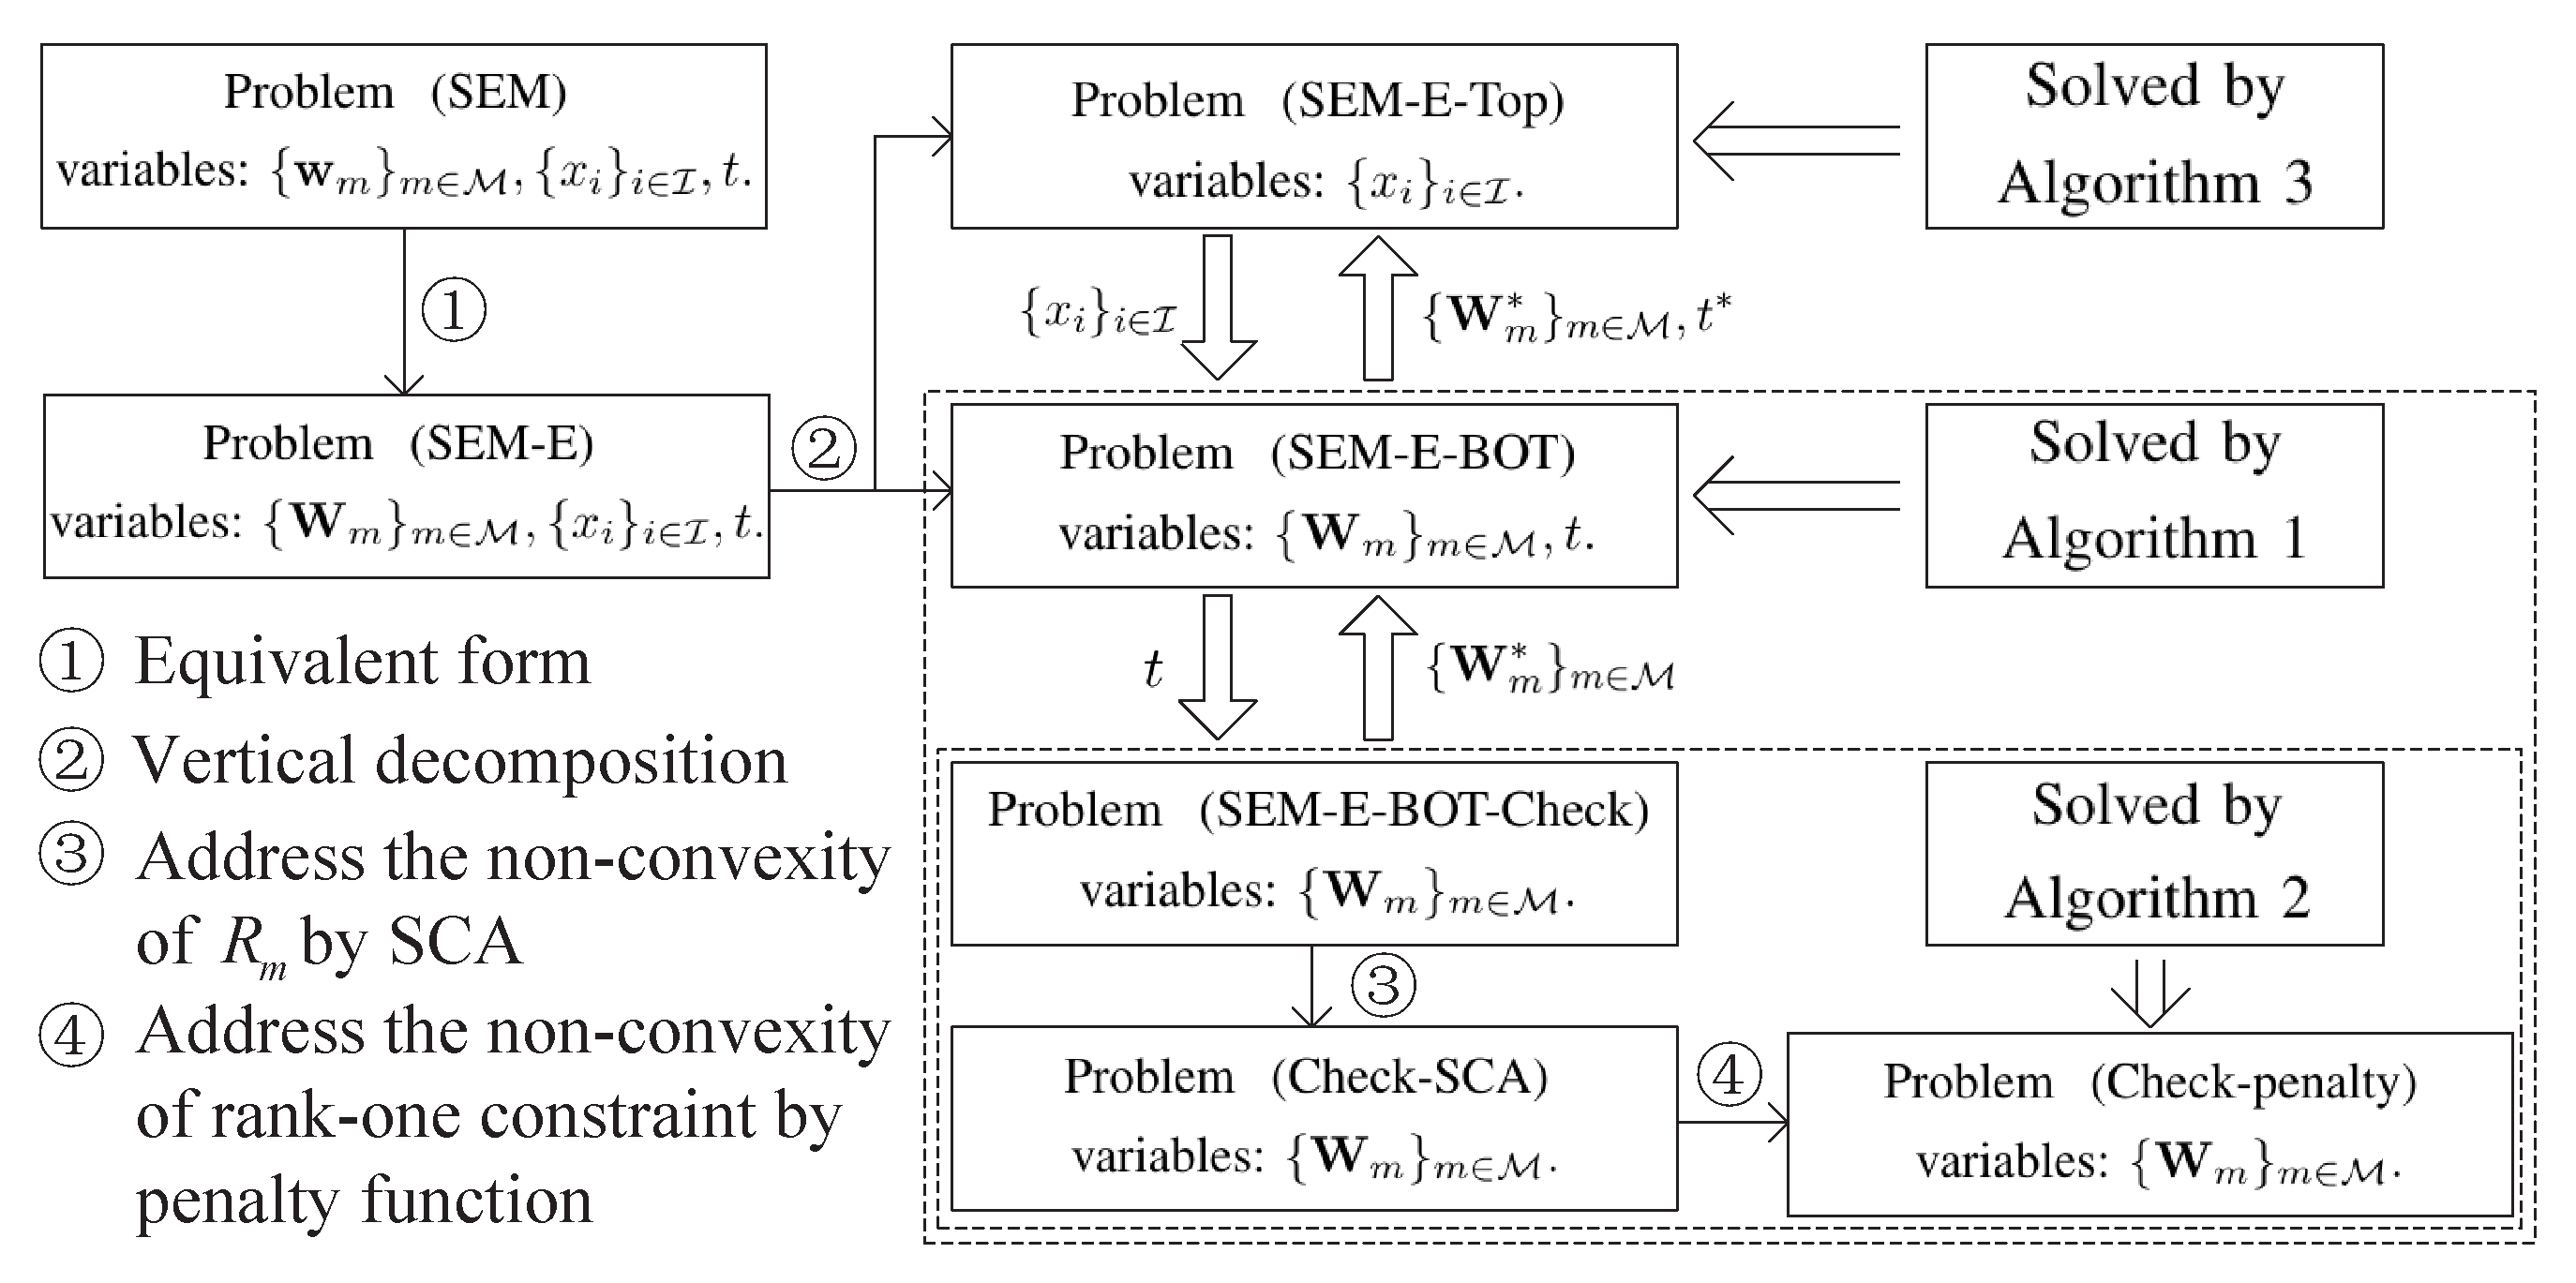
\includegraphics[width=0.6\textwidth]{figs_iotj_cld/Figure2.eps}
	\caption{Performance advantages under different numbers of SCDs}
	\label{chap4fig2}
\end{figure}
\begin{figure}
	\centering
	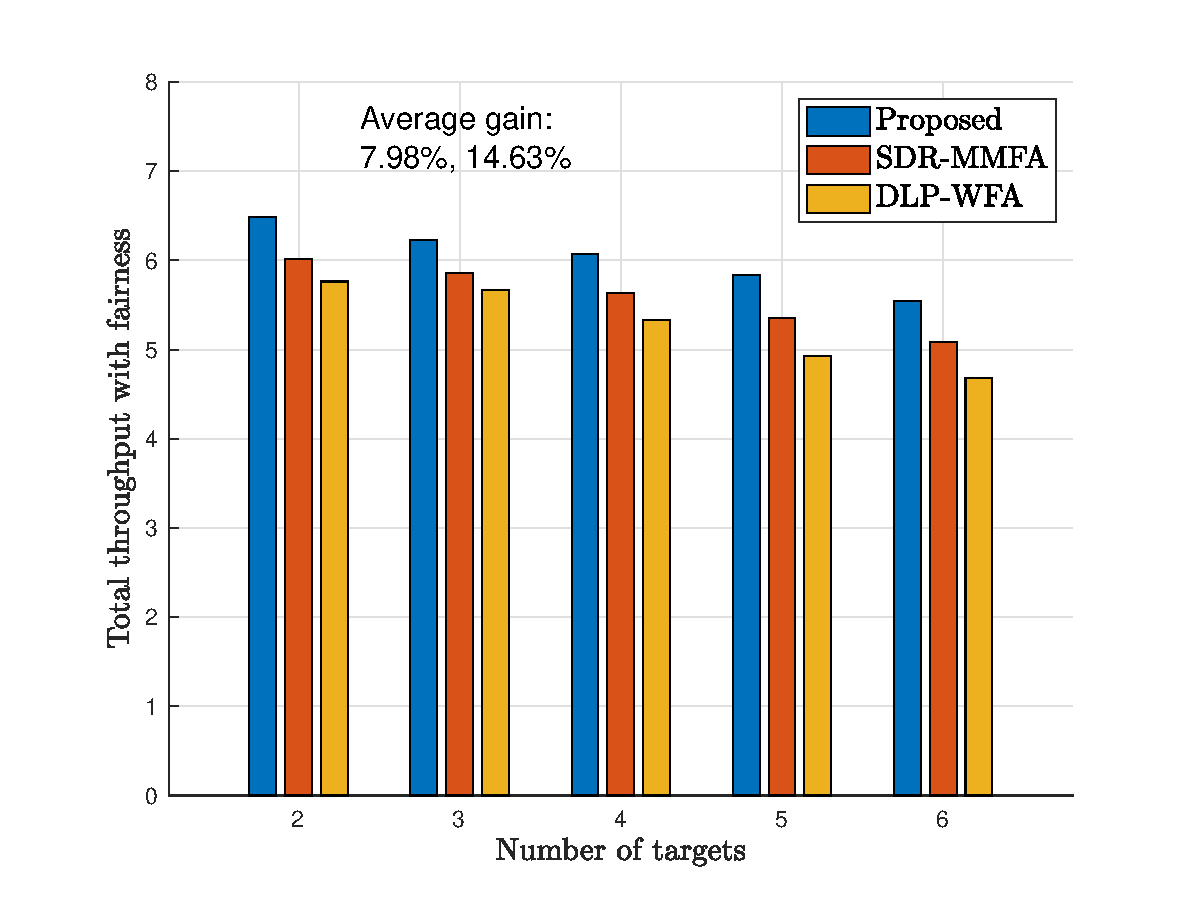
\includegraphics[width=0.6\textwidth]{figs_iotj_cld/Figure3.eps}
	\caption{Performance advantages under different numbers of targets}
	\label{chap4fig3}
\end{figure}

\begin{figure}
	\centering
	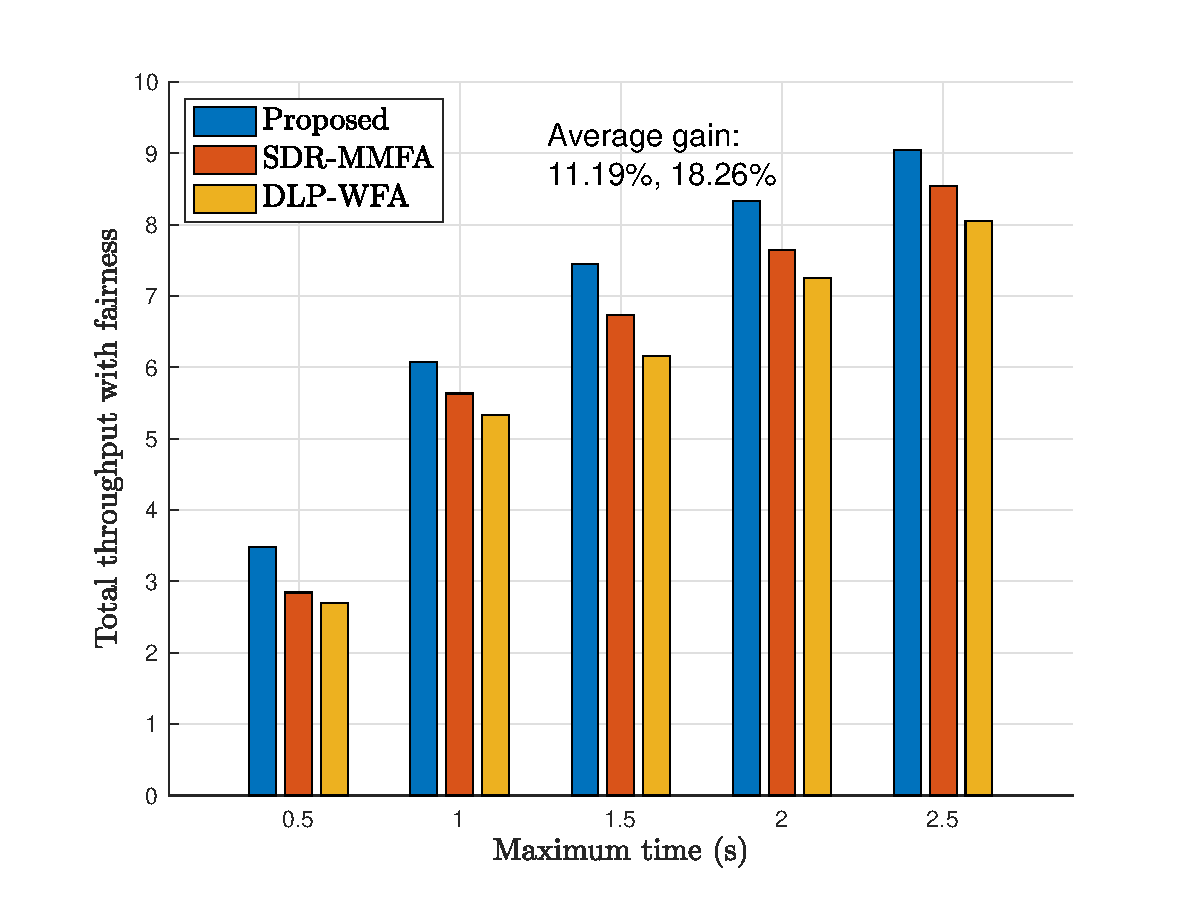
\includegraphics[width=0.6\textwidth]{figs_iotj_cld/Figure4.eps}
	\caption{Performance advantages under different values of the maximum time}
	\label{chap4fig4}
\end{figure}

\begin{figure}
	\centering
	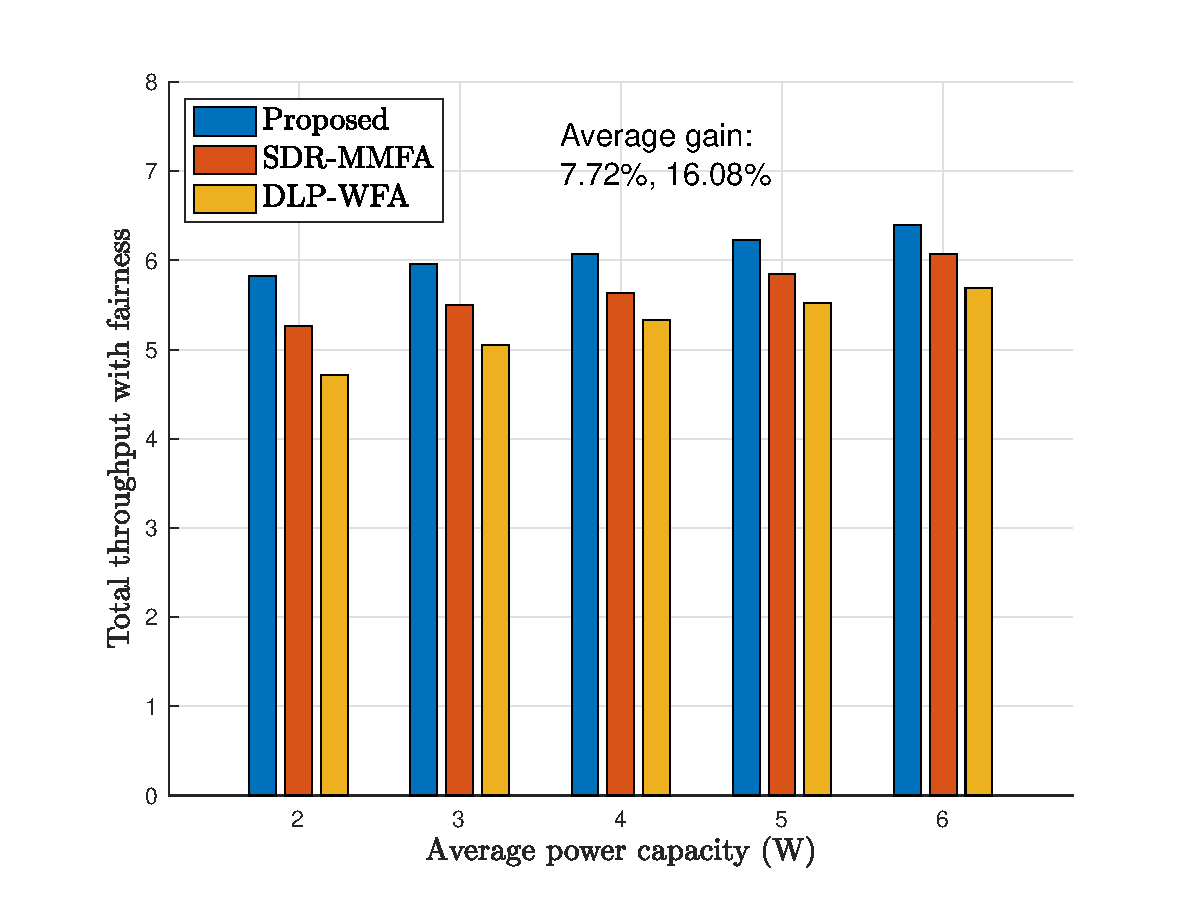
\includegraphics[width=0.6\textwidth]{figs_iotj_cld/Figure5.eps}
	\caption{Performance advantages under different values of the average power}
	\label{chap4fig5}
\end{figure}

\begin{figure}
	\centering
	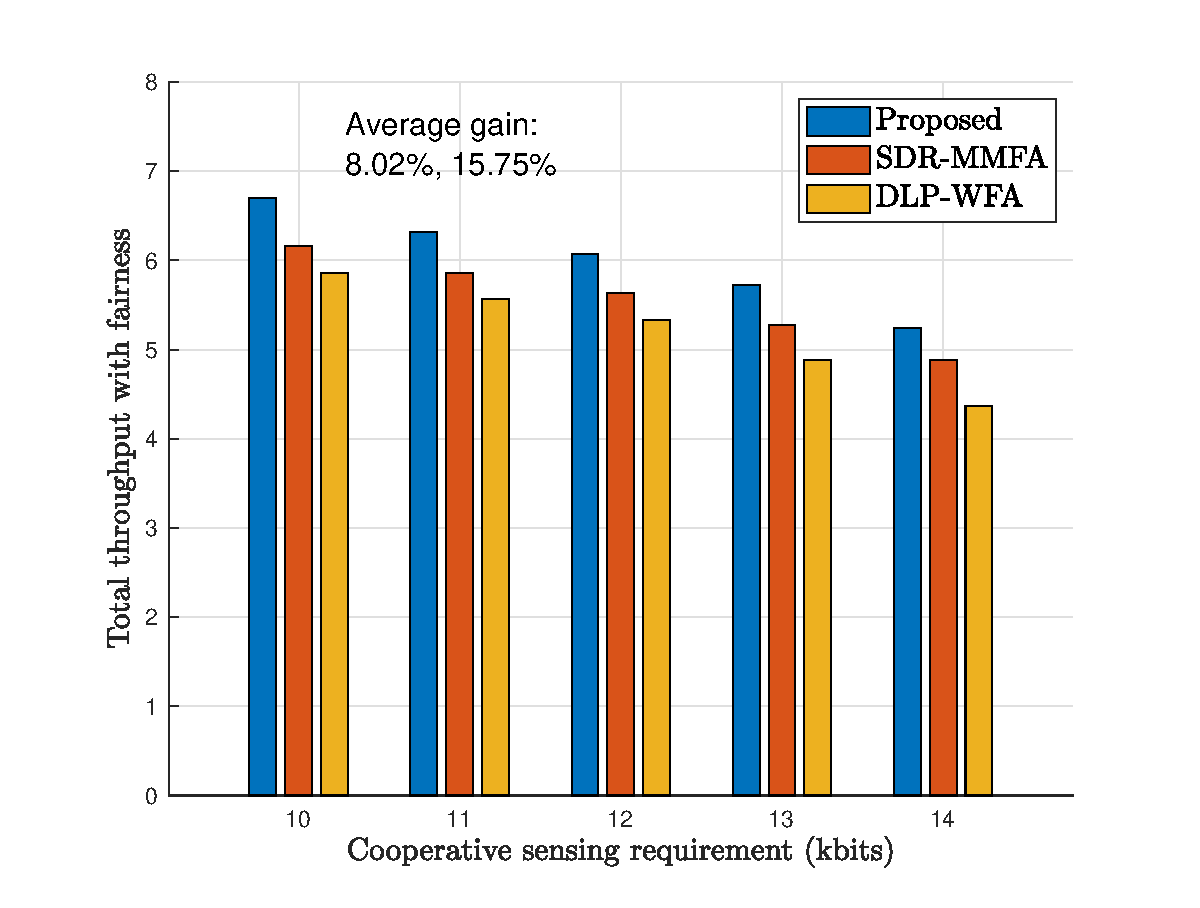
\includegraphics[width=0.6\textwidth]{figs_iotj_cld/Figure6.eps}
	\caption{Performance advantages under different cooperative sensing requirements}
	\label{chap4fig6}
\end{figure}

\begin{figure}
	\centering
	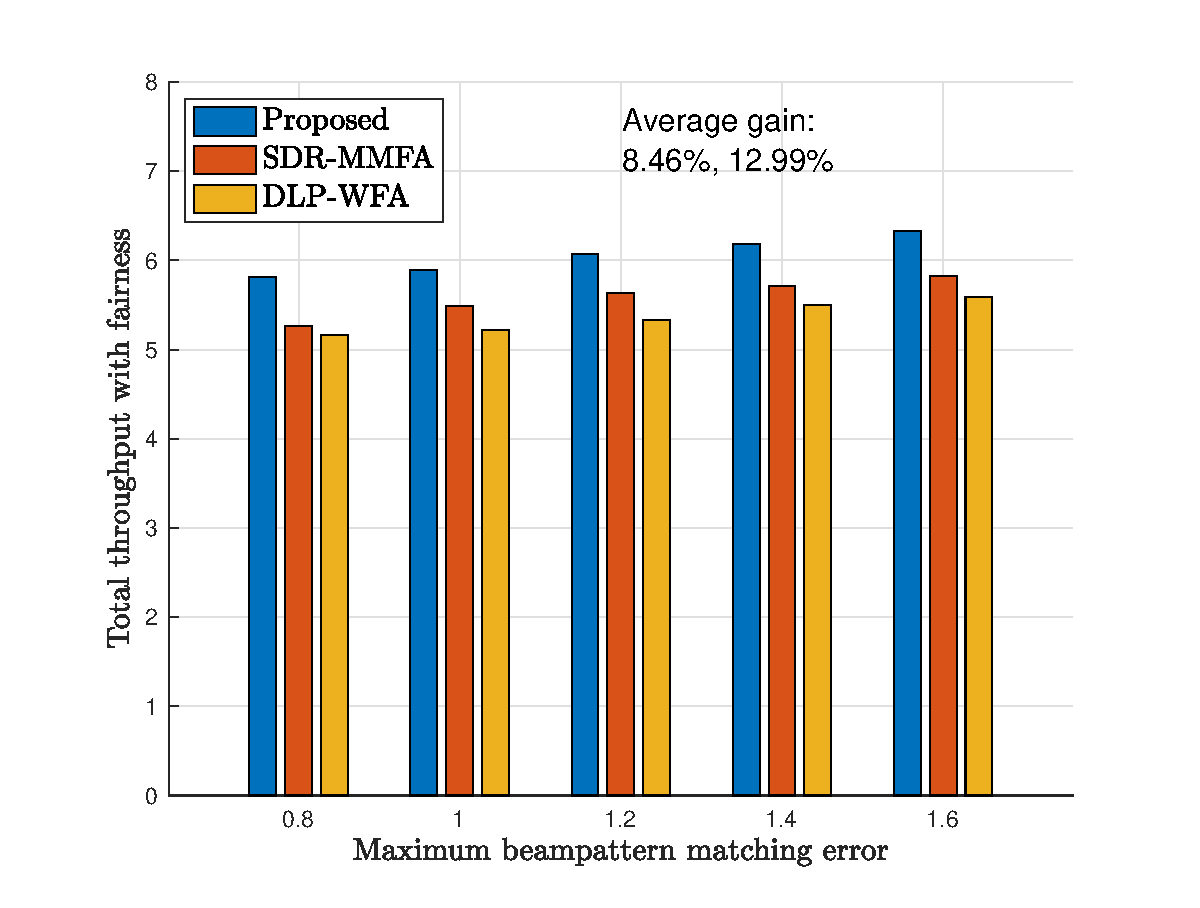
\includegraphics[width=0.6\textwidth]{figs_iotj_cld/Figure7.eps}
	\caption{Performance advantages under different values of the maximum multi-target sensing beampattern matching error}
	\label{chap4fig7}
\end{figure}

\subsection{Evaluation of the Fairness-aware Cooperative Sensing}
The comparison benchmark schemes are as follows.
\begin{itemize}
	\item FSSCS scheme: In full spectrum sharing cooperative sensing (FSSCS) scheme, the SCDs perform cooperative sensing towards multiple targets with full spectrum sharing and send data to the BS simultaneously, where each SCD suffers interference from other SCDs' signals.
	\item FDCCS scheme: In frequency division-based clustering cooperative sensing (FDCCS) scheme, the SCDs and targets are clustered into several clusters according to distance. Then, the SCDs perform cooperative sensing towards targets within the same cluster and send data to the BS simultaneously. Each cluster has a pre-assigned frequency band, and the frequency bands between different clusters are orthogonal to each other, and thus there is no co-channel interference between different clusters.
\end{itemize}





Figures \ref{chap4fig8} and \ref{chap4fig9} verify the performance advantages of the proposed fairness-aware cooperative sensing design. In Figure \ref{chap4fig8}, we plot the total throughput achieved by the schemes with different cooperative sensing requirements. In Figure \ref{chap4fig9}, we plot the total cooperative sensing quality achieved by the schemes with different maximum multi-target sensing beampattern matching errors. 
In particular, the average gains obtained by our proposed scheme over the benchmarks (i.e., FSSCS and FDCCS) are marked at the top of two figures.
Figures \ref{chap4fig8} and \ref{chap4fig9} demonstrate that our fairness-aware cooperative sensing scheme outperforms the benchmark schemes in both throughput and cooperative sensing accuracy.


\begin{figure}
	\centering
	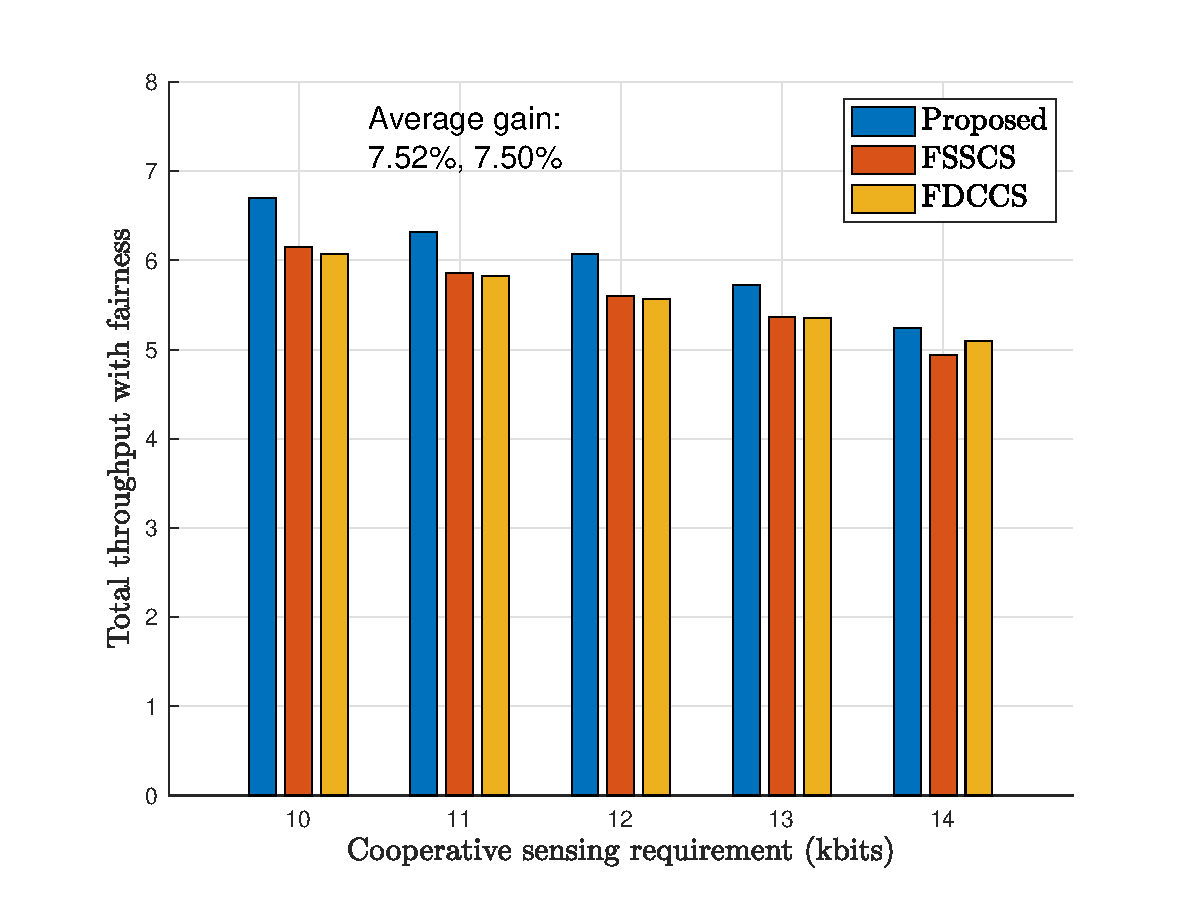
\includegraphics[width=0.6\textwidth]{figs_iotj_cld/Figure8.eps}
	\caption{Performance advantages of our fairness-aware cooperative sensing scheme in throughput}
	\label{chap4fig8}
\end{figure}

\begin{figure}
	\centering
	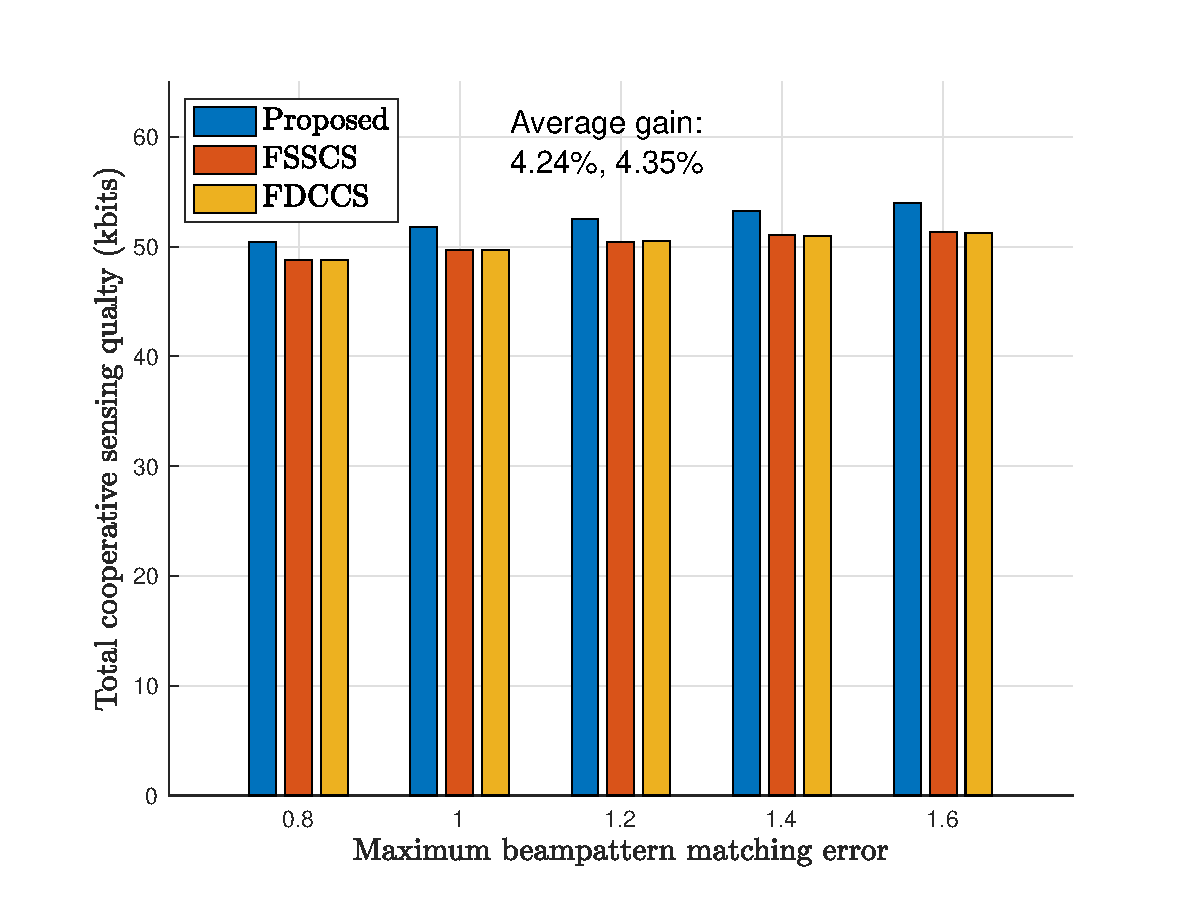
\includegraphics[width=0.6\textwidth]{figs_iotj_cld/Figure9.eps}
	\caption{Performance advantages of our fairness-aware cooperative sensing scheme in sensing accuracy}
	\label{chap4fig9}
\end{figure}

\begin{figure}
	\centering
	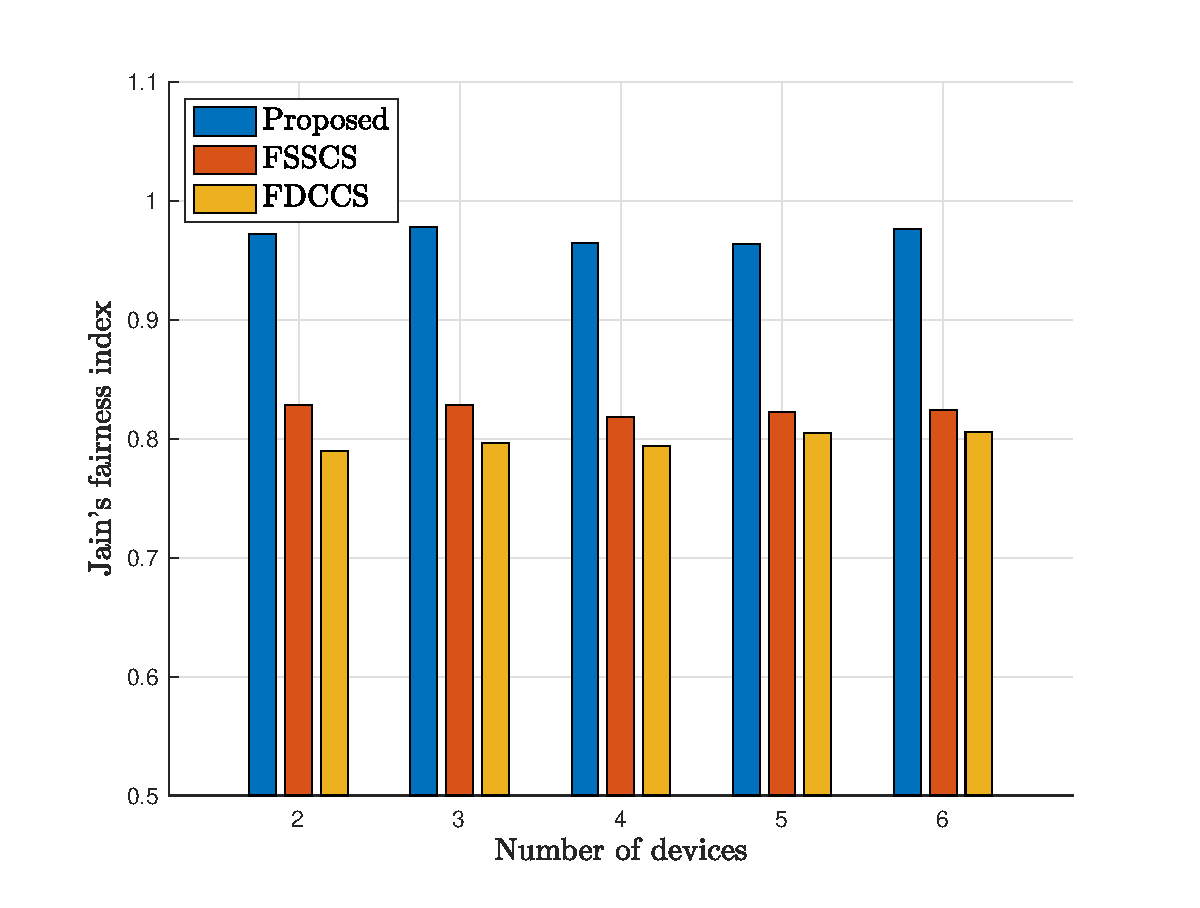
\includegraphics[width=0.6\textwidth]{figs_iotj_cld/Figure10.eps}
	\caption{Fairness advantages of our proposed cooperative sensing scheme}
	\label{chap4fig10}
\end{figure}



Figure \ref{chap4fig10} verifies the fairness advantages of our proposed cooperative sensing scheme. To evaluate the fairness performance, we use the metric of Jain's fairness index, which can quantifies the fairness in throughput achieved among SCDs \cite{iotj.jain1999throughput}. Jain's Fairness Index is defined as
\begin{equation}
	JFI(x_1,x_2,...,x_n)=\frac{(\sum_{i=1}^{n}x_i)^2}{n\sum_{i=1}^{n}x_i^2}.
\end{equation}
where $x_i$ denotes the achieved performance of the $i$-th SCD, and $n$ is the total number of SCDs. The index ranges from $\frac{1}{n}$ (the worst case) to 1 (the best case), with higher values indicating better fairness. It can be observed that our proposed cooperative sensing scheme outperforms the benchmark schemes in the data transmission fairness. The higher fairness index indicates that our approach allocates resources among devices in a more fairness manner and avoids significant differences in data transmission performance.

\section{Conclusion} \label{chap4_sec_conclusion}

In this chapter, we have proposed a fairness-aware design for ISAC-enabled multi-device cooperative sensing system, in which the SCDs engage in cooperative sensing towards multiple targets in a time-division manner while simultaneously delivering data to the BS. We have formulated a joint beamforming optimization for both sensing and transmission and the time allocation for different SCDs, aiming at maximizing the fair total throughput. To address its non-convexity, we have adopted a decomposition-based framework and identified the solution features of the decomposed subproblems. We further proposed an efficient algorithm for solving it. The numerical results validate the effectiveness of our proposed approach and demonstrate the performance advantages of our fairness-aware ISAC-enabled multi-device cooperative sensing in improving both the throughput and cooperative sensing accuracy. 